% research-report.tex: 调研报告
% Copyright (C) 2022 吴骏东, 张子辰, 蓝俊玮, 郭耸霄 and 陈建绿
% All rights reserved.

% This file is part of Runikraft. Runikraft is free software,
% which is released under the BSD 3-Clause License, see LICENSE for detail.
% Runikraft is provided ``as is'', without any express or implied warrenties.

% The reports of Runikraft are released under the Creative Commons
% Attribution 4.0 International License; see report/LICENSE for detail.
\documentclass[UTF8,fontset=none,linespread=1.15]{ctexart}
\ctexset
{
    section/format={\Large\sffamily\bfseries},
    subsection/format+={\sffamily},
    subsubsection/format+={\itshape}
}
\setCJKmainfont[ItalicFont={KaiTi},BoldItalicFont={KaiTi},
BoldItalicFeatures={FakeBold=3}]{Noto Serif CJK SC}
\setCJKsansfont[BoldFont={Noto Sans CJK SC Bold},
BoldItalicFont={Noto Sans CJK SC Bold},
AutoFakeSlant]{Noto Sans CJK SC DemiLight}
\setCJKmonofont[AutoFakeBold=3,AutoFakeSlant]{FangSong}
\setmainfont{cmun}[Extension=.otf,UprightFont=*rm,
ItalicFont=*ti,BoldFont=*bx,BoldItalicFont=*bi]
\setsansfont{cmun}[Extension=.otf,UprightFont=*ss,
ItalicFont=*si,BoldFont=*sx,BoldItalicFont=*so]
\setmonofont{cmun}[Extension=.otf,UprightFont=*btl,
ItalicFont=*bto,BoldFont=*tb,BoldItalicFont=*tx]
%Computer Modern Unicode 的\textasciitilde和\~{}的高度相同,所以用\tildechar表示居中的波浪线~
\newcommand{\tildechar}{\raisebox{-0.35em}{\textasciitilde}}
\usepackage[a4paper,hmargin=1.2in,vmargin=1in]{geometry}
\usepackage{graphicx,tikz,float,subfig,multicol,makecell,multirow,longtable}
\usepackage{verbatim}
\usepackage[normalem]{ulem}
\usepackage{CJKfntef}
\usepackage[perpage]{footmisc}

%目录, 参考了OSH-2021/x-sBPF
\usepackage{titletoc}
\titlecontents{section}[2em]{\addvspace{1.3mm}\bfseries}{%
\contentslabel{2.0em}}{}{\titlerule*[5pt]{$\cdot$}\contentspage}
\titlecontents{subsection}[4.2em]{}{\contentslabel{2.5em}}{}{%
\titlerule*[5pt]{$\cdot$}\contentspage}
\titlecontents{subsubsection}[7.2em]{}{\contentslabel{3.3em}}{}{%
\titlerule*[5pt]{$\cdot$}\contentspage}

%代码环境
\usepackage{listings}
\lstset{basicstyle={\normalfont\ttfamily},breaklines,tabsize=4}

\usepackage{enumitem}
\setlistdepth{5}
\renewlist{enumerate}{enumerate}{5}
\setlist{itemsep=0pt,partopsep=0pt,parsep=0pt,topsep=0pt}
\setlist[enumerate,1]{label=\arabic*.}
\setlist[enumerate,2]{label=(\arabic*)}
\setlist[enumerate,3]{label=\textcircled{\arabic*}}
\setlist[enumerate,4]{label=(\textit{\roman*})}
\setlist[enumerate,5]{label=\textit{\alph*})}

\usepackage[colorlinks,unicode,pdfstartview={FitH}]{hyperref}
\hypersetup
{
  pdftitle={2022春 操作系统原理与设计(H) x-runikraft小组 调研报告},
  pdfauthor={吴骏东; 张子辰; 蓝俊玮; 郭耸霄; 陈建绿}
}

%带圈数字,它必须在hyperref之后载入
\usepackage{xunicode-addon}
\makeatletter
\xeCJKDeclareCharClass{CJK}{"24EA, "2460->"2473, "3251->"32BF,"24B6->"24E9,"2160->"217F}
\newfontfamily\EnclosedNumbers{Noto Serif CJK SC}
\AtBeginUTFCommand[\textcircled]{\begingroup\EnclosedNumbers}
\AtEndUTFCommand[\textcircled]{\endgroup}
\makeatother

\makeatletter
\let\textcircled@old\textcircled
\protected\def\textcircled#1{%
	\expandafter\textcircled@old\expandafter{\expanded{#1}}}
\makeatother
\makeatletter
\renewcommand\@makefntext[1]{%
	\setlength\parindent{0.75\ccwd}\selectfont
	\@thefnmark\ #1}
\makeatother
\renewcommand*\thefootnote{\textcircled{\arabic{footnote}}}
\renewcommand{\lstlistingname}{代码}

%上标+引用
\let\nosupcite\cite
\renewcommand*{\cite}[1]{\textsuperscript{\nosupcite{#1}}}

%章节作者
\newcommand{\sectionauthor}[1]{%
\vspace*{-5ex}
\noindent\textrm{\hfill\textit{by #1}}
\vspace*{2ex}\par}
%\renewcommand{\today}{2022年4月8日}

\begin{document}
\sffamily %为方便屏幕阅读,文档主要使用无衬线字体
\title{\bfseries Runikraft小组\quad 调研报告}
\author{吴骏东\and 张子辰\and 蓝俊玮\and 郭耸霄\and 陈建绿}
\date{\today}
\maketitle

\tableofcontents

\section{项目简介}
Runikraft 是用Rust语言编写的能在RISC-V架构 + QEMU平台上运行unikernel。
它基于用C语言实现的Unikraft,在继承Unikraft的高效性、可定制性、良兼容性、
安全性的同时,进一步简化了构建系统镜像的流程,加入了RISC-V支持,并且
用Rust语言提供了更强的内核安全保证。
\section{项目背景}
\subsection{操作系统的架构}
\subsection{虚拟化}
\subsubsection{虚拟机}
\subsubsection{沙盒}
\subsubsection{Unikernel}
\subsection{Unikernel的研究与发展}
\subsubsection{Unikernel面临的问题}
\subsubsection{Unikernel的架构}
\subsection{知名的Unikernel项目}\label{subsec:famous-unikernel-projects}
本小节简要介绍我们详细了的六个近两年仍然在维护unikernel项目。在下面的介绍中,我们假定读者对
unikernel已经有了基本的认知,因此我们略去了unikernels都具有的特性,比如启动时间短、
镜像小、延迟低、用在云计算领域。

\subsubsection{ClickOS}\sectionauthor{蓝俊玮}

ClickOS 是一个基于 Xen 的高性能的虚拟化软件中间盒平台。为了达到高性能,
ClickOS 对 Xen 的 I/O 子系统实现了广泛的翻修,包括对后端交换机、
虚拟网络设备和后端前端驱动程序。这些更改使 ClickOS 能够显著加快中间盒运行时的网络连接。\cite{bib:12-clickos}

ClickOS 虚拟机只有5MiB ,启动仅需要大约30ms,而且延迟只有45µs。
ClickOS 实现了广泛的中间盒,包括防火墙、运营商级 NAT 和
负载均衡器,并证明 ClickOS 可以每秒处理数百万个数据包,达到生产级性能。\cite{bib:12-clickos}\cite{bib:13-clickos2}

\begin{figure}[!hbt]
\begin{minipage}{0.49\linewidth}
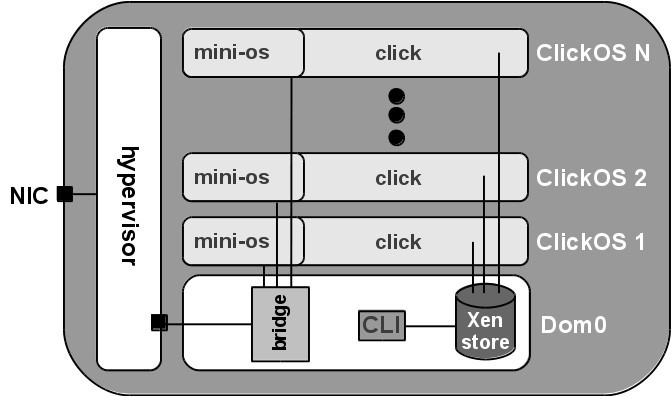
\includegraphics[width=\linewidth]{pictures/clickOS_arch.jpg}
\caption{ClickOS 的架构\cite{bib:13-clickos2}}
\end{minipage}
\begin{minipage}{0.49\linewidth}
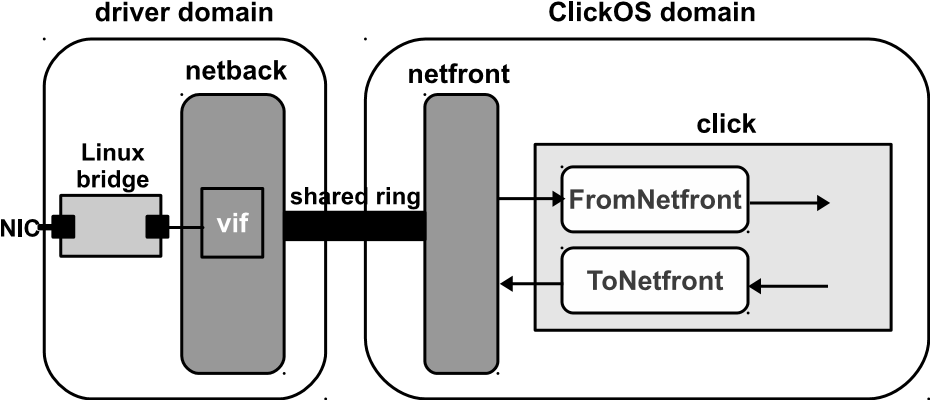
\includegraphics[width=\linewidth]{pictures/ClickOS_networking.png}
\caption{Basic ClickOS networking in Xen\cite{bib:12-clickos}}
\end{minipage}
\end{figure}

\subsubsection{MirageOS}\sectionauthor{蓝俊玮}

MirageOS 是一个用 OCaml 语言编写的,
用于在各种云计算和移动平台构建安全、高性能网络应用程序的库操作系统。
它可以将大型服务器划分为很多更小的虚拟机,使得服务器具有更强的拓展性和安全性。
其代码可以在 Linux 、Mac OS 等系统中开发,然后编译成一个完全独立的、专门的内核,
可以在 Xen、KVM hypervisors 或轻量级 hypervisors 下运行。MirageOS
已经发展成为一个由近100个开放源码库组成的成熟库,实现了一系列广泛的功能,
并且正开始与 Citrix XenServer 等商业产品集成。MirageOS
将 Xen hypervisors当成一个稳定的硬件平台,让我们可以专注于实施高性能协议,
没必要为支持传统操作系统里面的成千上万个设备驱动程序而操心。\cite{bib:11-unikerel2}

\begin{figure}[!hbt]
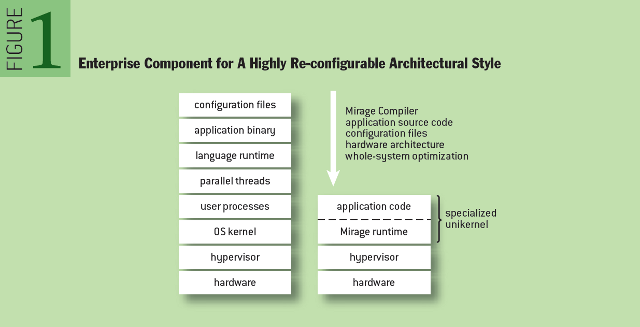
\includegraphics[width=\linewidth]{pictures/figure1.png}
\caption{MirageOS 的架构}\label{fig:mirage-fig1}
\end{figure}

\begin{figure}[!hbt]
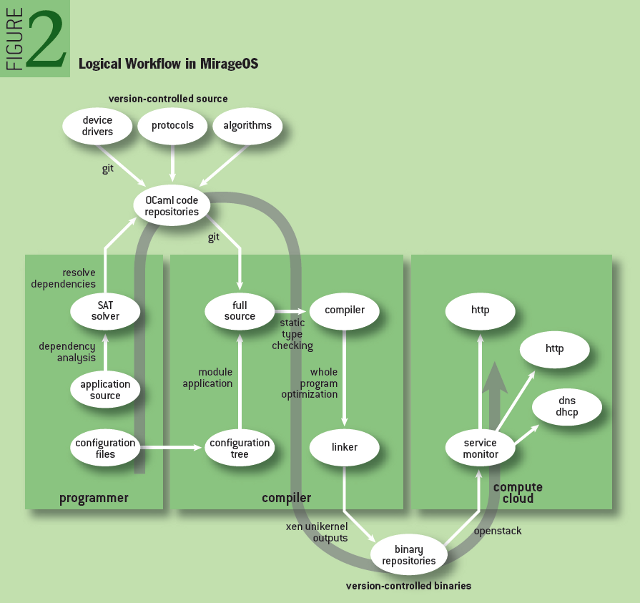
\includegraphics[width=\linewidth]{pictures/figure2.png}
\caption{MirageOS的逻辑工作流}\label{fig:mirage-fig2}
\end{figure}

MirageOS的亮点是输入应用程序的所有源代码依赖项都被显式跟踪,包括实现内
核功能所需的所有库。MirageOS 包括一个构建系统,该系统内部使用
一个 SAT 解算器(使用 OPAM 包管理器,使用 Mancoosi 项目的解算器)
从一个已发布的在线包集中搜索兼容的模块实现。由于 OCaml 的静态类型
检查,在编译时将捕获接口中的任何不匹配。

在 MirageOS 中,OCaml 编译器接收整个内核代码的源代码,
并将其链接到一个独立的本机代码对象文件。它链接到提供引导支持和
垃圾回收器的最小运行时。没有抢占式线程,内核是通过一个 I/O 循环轮询
Xen 设备的事件驱动的。\cite{bib:11-unikerel2}

\subsubsection{IncludeOS}\sectionauthor{蓝俊玮}

IncludeOS 是一个为开发基于 unikernel 的应用程序而创建 C++ API 的项目。\cite{bib:9-includeos}

当 IncludeOS 映像引导时,它通过设置内存、运行全局构造函数、注册驱动程序和中断处理
程序来初始化操作系统。IncludeOS 不支持虚拟内存,应用程序和
 unikernel 库使用单个地址空间。因此,没有系统调用或用户空间的概念; 所有操作系统服务
 都通过对库的简单函数调用来调用,并且都以特权模式运行。\cite{bib:10-includeos2}

\noindent IncludeOS 有如下优点:\cite{bib:9-includeos}
\begin{itemize}
\item IncludeOS中目前没有进程抢占,所以操作系统的行为非常静态。
只要机器本身是可预测的,延迟也将是完全可预测的。因此,在裸机硬件上,
IncludeOS可被视为低延迟,可预测的操作系统。
\item 对网络的支持很好,与 Linux 相比表现出色。
\item IncludeOS 系统作为一个整体进行编译和优化。在编译器和连接器阶段,
优化器可以更多地了解整个系统正在做什么,并且有可能进一步优化。
\item IncludeOS 中的所有 IRQ 处理程序将简单地(原子地)更新计数器,
并在有时间时将进一步的处理推迟到主事件循环。这消除了对上下文切换的需要,
同时也消除了与并发相关的问题,如竞争条件。
通过使所有 I/O 都是异步的,CPU 保持忙碌,这样就不会发生阻塞。
\end{itemize}

\noindent IncludeOS 有如下缺点:\cite{bib:9-includeos}
\begin{itemize}
\item IncludeOS 不实现所有 POSIX。开发人员认为,
只有在需要时才会实现 POSIX 的某些部分。开发人员不太可能将完全遵守 POSIX 作为一个目标。
\item 与MirageOS一样,IncludeOS 中没有实现阻塞调用,因为当前的事件循环模型是使用它的最佳方式。
\item IncludeOS 目前还缺少可写的文件系统。
\end{itemize}

\subsubsection{RustyHermit}\sectionauthor{陈建绿}

RustyHermit(\href{https://github.com/hermitcore/rusty-hermit}{Github}) 是
一个基于 Rust 的、轻量级的 Unikernel,也是一个用来评估操作系统新的设计的研究项目。
它用 Rust 语言完全改写了 RWTH Aachen University
 开发的研究项目 \href{http://hermitcore.org/}{HermitCore}\footnote{HermitCore 最初是用 C 语言编写的,是一种针对高性能和云计算的可伸缩和可预测的运行时的 Unikernel。}。\cite{bib:14-rusty-hermit}

该项目完全使用 Rust 语言开发,Rust 的所有权模型保证了它的内存/线程安全,
并且让开发者能够在编译时就消除许多种 bug。因此,与通用编程语言相比,使用 Rust
 进行内核开发会留下更少的漏洞,得到更加安全的内核。

开发者扩展了 Rust 工具链以至于 RustyHermit 的 build 过程
与 Rust 通常的工作流程相似。使用 Rust runtime 而且不直接使用 OS 服务的
 Rust 应用程序能够直接在 RustyHermit 上运行而不需要修改。因此,原则上,
 每一个现有的 Rust 应用程序都可以建立在 RustyHermit 之上。\cite{bib:17-rusty-hermit2}


RustyHermit 中优化实现了网络栈。它使用 \href{https://github.com/smoltcp-rs/smoltcp}{smoltcp}
作为它的网络栈,使用 \href{https://www.linux-kvm.org/page/Virtio}{Virtio}
作为客户机和主机操作系统之间的接口。
%将RustyHermit 和 Linux 分别作为客户端运行在基于 Linux 的主机系统上的虚拟机中,以信息的比特数作为自变量,吞吐量/Mbps作为因变量,
%进行测试并绘图,结果如下:\cite{bib:20-linux-kernel}
%\begin{figure}[H]
%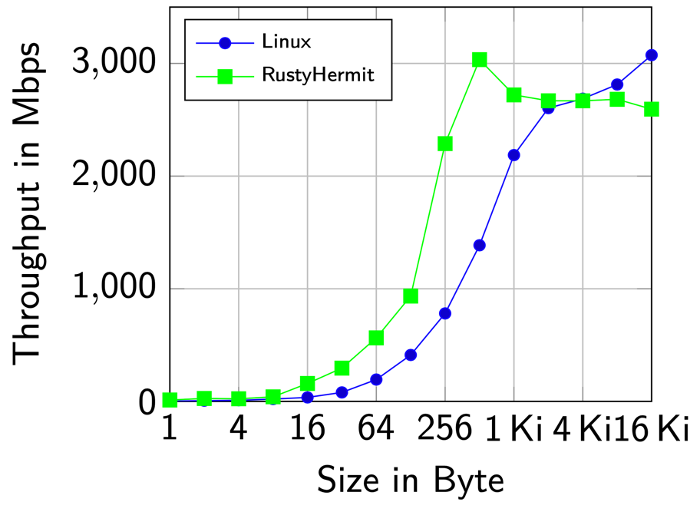
\includegraphics[width=\linewidth]{pictures/RustyHermit-1.png}
%\caption{}
%\end{figure}
%
%由结果图可以看出,\textbf{RustyHermit 在信息比特数较小时吞吐量明显比 Linux 更快}。

Sung, Olivier, Lankes and Ravindran\cite{bib:18-intra-unikernel}
提出了一个修改版本的 RustyHermit,该版本利用Intel MPK(Memory Protection Keys)\cite{bib:19-mpk},
在保持单一地址空间的同时,在 Unikernel 实例中引入内存隔离,
包括安全内核代码与不安全内核代码之间的隔离、内核代码与用户代码之间的隔离。
在一组宏基准测试中,带有隔离功能的 unikernel 仅减慢了0.6\%。

这篇论文中的内容可以作为我们实现 runikraft 的参考。

\subsubsection{Rumprun}\sectionauthor{陈建绿}

Rumprun unikernel 是在 rump kernels 的基础上开发的。
Rumprun 不仅可以在像 KVM 和 Xen 这样的管理程序上工作,
还可以在裸金属上工作。无论有没有 POSIX-y 接口,Rumprun 都
可以正常使用。如果有 POSIX-y 接口,Rumprun 则允许现有的、
未经修改的 POSIX 应用程序开箱即用;如果没有 POSIX-y 接口,
Rumprun 则允许构建高度自定义的解决方案,并且占用的空间最小。

Rumprun unikernel 支持用 C、 C++ 、 Erlang、 Go、
Java、 Javascript (node.js)、 Python、 Ruby 和 Rust 等语言编写的应用程序。

在 \href{https://github.com/rumpkernel/rumprun-packages}{rumprun-packages repository}
中可以找到用于 Rumprun 的现成软件包,比如 \texttt{LevelDB},
\texttt{Memcached}, \texttt{nanomsg}, \texttt{Nginx} 和 \texttt{Redis}。

\paragraph{1. Rump kernels 的相关介绍}\cite{bib:21-rump-kernel}\cite{bib:22-xen}

Rump kernels 的组件来自未经修改的 NetBSD,由此开发者提供了一个 POSIX-y API。
Rump Kernel 项目以一种可用于构建轻量级、特殊用途虚拟机的形式提供了 NetBSD 的
模块化驱动程序。因为开发者没有做会将错误引入到应用程序运行时(application runtime)、
libc 或驱动程序中的移植工作,所以程序可以很稳定地工作。
\begin{figure}[!hbt]
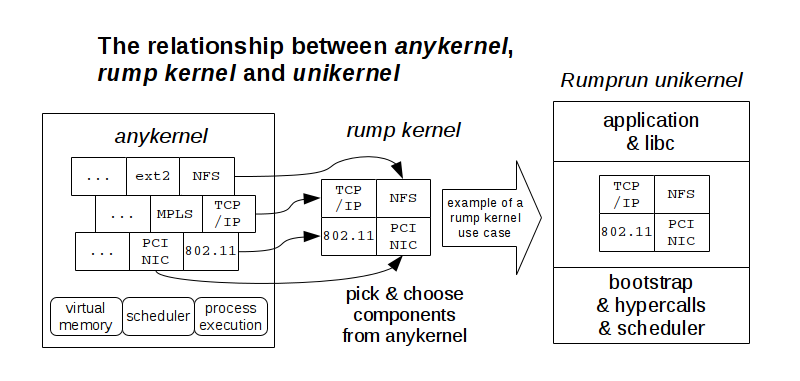
\includegraphics[width=\linewidth]{pictures/rumprun-1.png}
\caption{Anykernel、
Rump kernel 和 Rumprun Unikernel 的关系}
\end{figure}

\begin{quote}
“Anykernel”概念指的是一种与架构无关的驱动程序方法,在这种方法中,驱动程序既可以编译到宏内核中,也可以作为用户空间进程运行,具有微内核风格,并且不需要修改代码。\\
\hspace*{\fill}——维基百科
\end{quote}

\paragraph{2. Rumprun 的相关介绍}\cite{bib:23-mirageos}\cite{bib:24-rumrun}

Rumprun 可用于将几乎任何与 POSIX 兼容的程序转换为一个可工作的
Unikernel。使用 Rumprun,理论上可以将 Linux 或者 类Unix系统上的大部分
程序编译成 Unikernel。Rumprun 以开发 NetBSD 内核中的驱动程序并在用户空间
中进行测试的需求为出发点,主要的工作是重构这个代码库,使其看起来像一个库操作系统。

\begin{figure}[!hbt]
\begin{minipage}{0.49\linewidth}
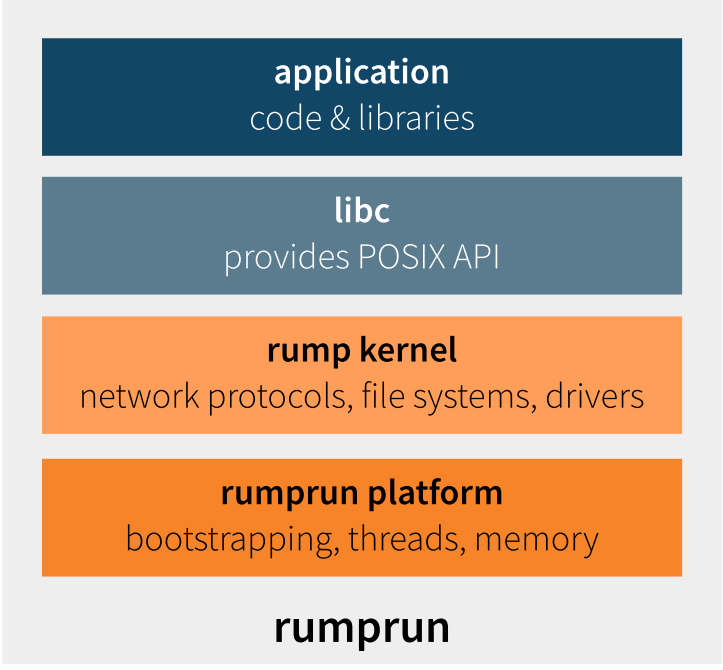
\includegraphics[width=\linewidth]{pictures/rumprun-2-cut.png}
\caption{Rumprun 的架构}
\end{minipage}
\begin{minipage}{0.49\linewidth}
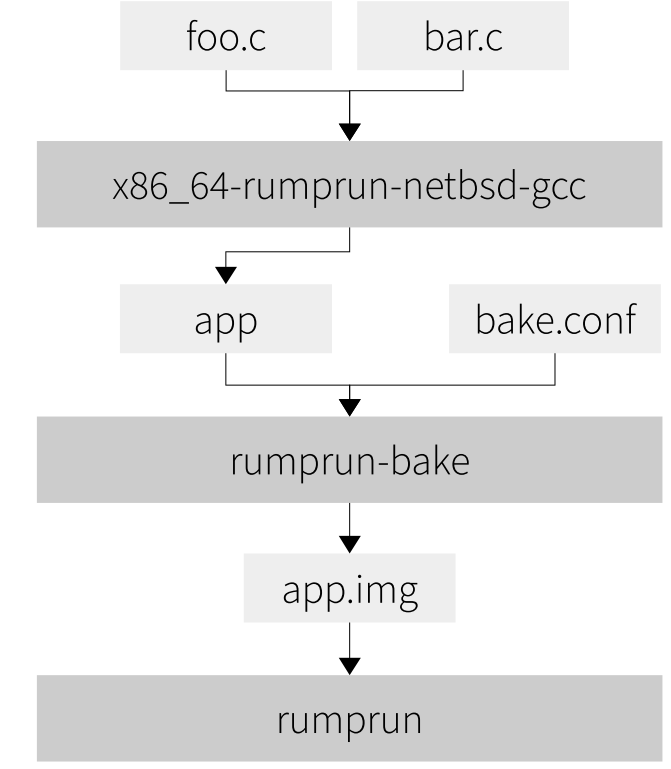
\includegraphics[width=\linewidth]{pictures/rumprun-3-cut.png}
\caption{Rumprun 的工作流程示例}
\end{minipage}
\end{figure}

Rumprun 也有一些限制:

\begin{itemize}
\item single address-space
    \begin{itemize}
    \item no processes
    \item no virtual memory
    \item no signals
    \end{itemize}
\item toolchain
    \begin{itemize}
    \item still experimental
    \end{itemize}
\item threading
    \begin{itemize}
    \item cooperative
    \item single-core
        \begin{itemize}
        \item need to spawn multiple unikernels to use multiple cores
        \end{itemize}
    \end{itemize}
\end{itemize}

我在调研的过程中发现,rump kernel 的好多官方文档都会重定向到
\url{https://rumpkernel.org}这个网址,而这个网址目前只有一些 IT News,
并非和 rump kernel 相关的内容,所以\textit{猜测该项目目前已经无人维护}。

\subsubsection{Nanos}\sectionauthor{陈建绿}

我在调研过程中发现一个比较新的正在开发中的 Unikernel:\href{https://github.com/nanovms/nanos}{Nanos(Github)}。下面是它的一些介绍:

\begin{itemize}
\item Nanos 是一个新的内核,旨在虚拟化环境中运行一个且仅有一个应用程序。
与 Windows 或 Linux 等通用操作系统相比,它有几个限制——即它是一个单进程系统,
不支持运行多个程序,也不具备通过 ssh 进行用户或远程管理的概念。
\item Nanos 的目标是成为一个比 Linux 安全得多的系统。
它做到这一点的几个依赖:没有用户的概念,每个虚拟机只运行一个进程,限制每个虚拟机中包含的代码数量。
\item Nanos 并不打算在裸金属上运行,所以开发者努力使其内核\textit{尽可能简单}。
\end{itemize}

这也许会对我们的项目有所帮助。

\subsubsection{Unikraft}\sectionauthor{张子辰}
Unikraft是一个比较新的unikernel。可以说,它在设计时就充分考虑
了现有的unikernels的优缺点。它在保持unikernel的极简化、
高效的同时,兼容了完整的POSIX兼容层,使开发者可以轻松地将现有的为Linux
编写的代码移植到unikernel上。Unikraft由若干低耦合的模块组成,内存分配器、
调度器、网络栈、引导代码都是独立的微型库。Unikraft的API即为微型库本身,
这意味着可以在生成时轻松地添加或移除APIs。\cite{bib:unikraft}

Unikraft遵从如下设计原则:
\begin{itemize}
\item 内核应该是完全模块化的,以便允许unikernel被彻底而轻松的定制。
在Unikraft中,内存分配器、调度器、网络栈、引导程序等系统原件都是
独立的微型库。
\item 内核应该提供注重效率、良定义的API,而且允许用户轻松地
为了满足自己的程序的性能要求选择、组装它们。在Unikraft中,这些APIs
就是微型库本身,这意味着它们可以轻松地在构建时增减,而且提供更多
的微型库即可拓展它们功能。
\end{itemize}

目前,Unikraft已经SQLite, nginx, Redis等程序,C/C++, Go, Python, Ruby,
Web Assembly and Lua等编程语言或运行环境。

在架构方面,Unikraft融合了宏内核的单地址空间带来的高效性和微内核的模块化带来的
可拓展性。OS的功能被分割成若干细粒子度的组件,而各个组件之间通过良定义的APIs
通信。Unikraft用精心设计的APIs和静态链接获得高效率,而不是为了效率破坏API
的边界。Unikraft大致分为两部分:
\begin{itemize}
\item \textbf{微型库}:微型库是实现一部分的Unikraft的APIs的软件组件,
Unikraft的作者有意将它们分割到了不同的库中,并尽可能降低它们之间的依赖。
实现相同APIs的微型库可以相互替换。比如,Unikraft内核就提供了多种实现
\texttt{ukalloc}接口的内存分配器。
\item \textbf{构建系统}:它为用户提供基于Kconfig的配置菜单\footnote{在实验1中,
我们在定制Linux内核时,运行\texttt{make menuconfig}后看到的就是Kconfig菜单。},
用户可用它选择要用哪些微型库,要为哪个平台和哪个CPU架构构建。
\end{itemize}
\begin{figure}[!hbt]
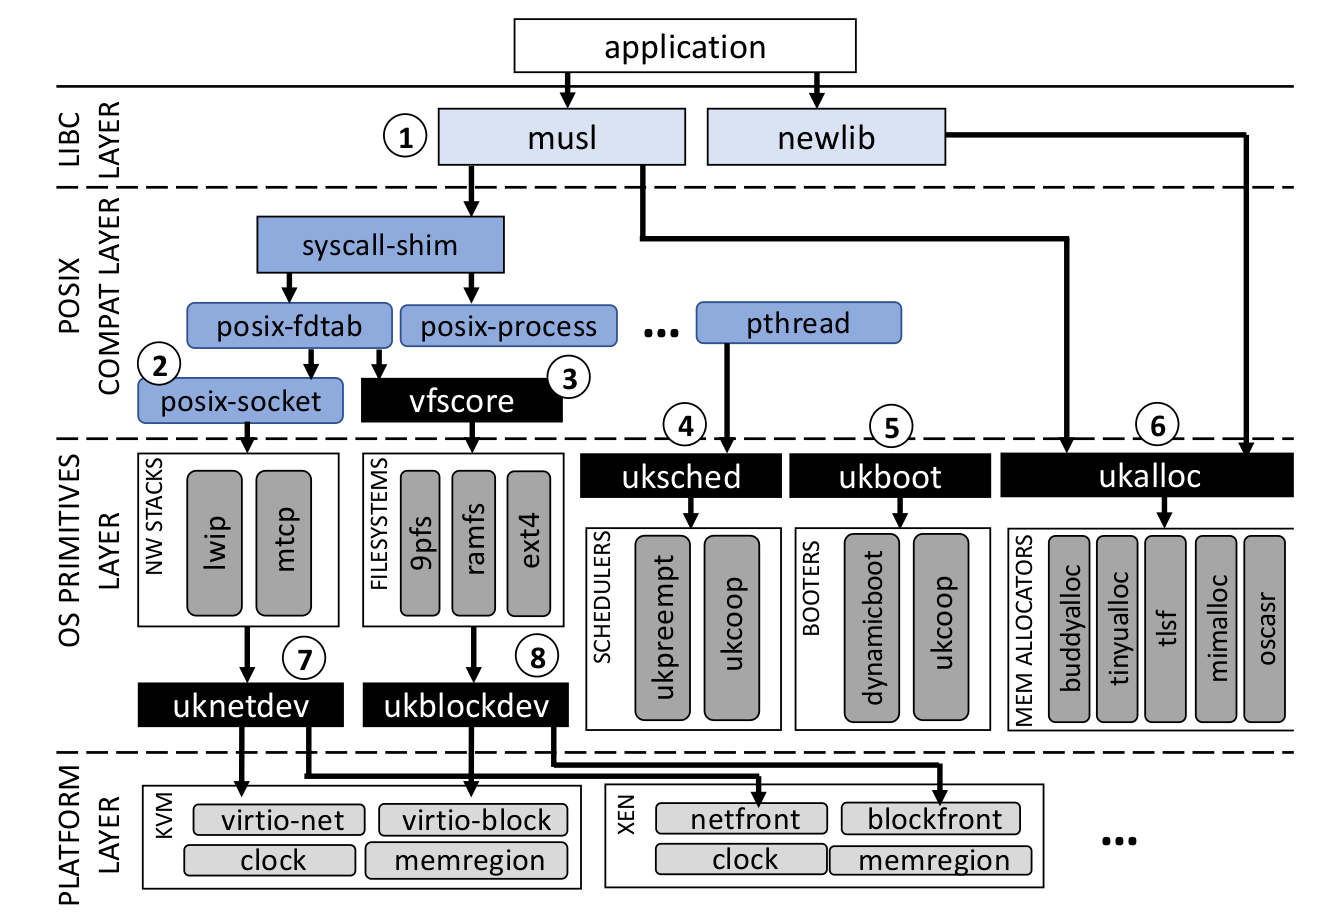
\includegraphics[width=\linewidth]{pictures/Unikraft-architecture.png}
\caption{Unikraft的架构(黑色框内的是APIs)允许用户程序接入不同层次的APIs,也
允许用户选择不同的API实现。}\label{fig:unikraft-arch}
\end{figure}

图\ \ref{fig:unikraft-arch}\ 展示了Unikraft的架构。使用不同层次的APIs和
替换API实现的能力给开发者提供了多种优化可能。首先,未经修改的程序(如用C语言
写的Hello World和nginx)可以使用\texttt{musl}(图\ \ref{fig:unikraft-arch}\ 的①)
或\texttt{nolibc}提供的POSIX兼容层,并自动获得低启动时间、低内存消耗和
更高的吞吐量,因为在Unikraft中,系统调用是高效的函数调用。

类似地,程序的开发者可以轻松选择合适的内存分配器(⑥)以达到最高效率,甚至
在同一个unikernel中使用多种分配器(如为引导程序选择简单、快速的内存分配器,
并为程序本身选用默认分配器)。

关注快速引导的开发者也可以使用自己的遵守\texttt{ukboot} API的引导代码(⑤)。
对于网络密集型程序,开发者可以使用标准的套接字接口(②),或者使用更底层、更高效
的\texttt{uknetdev} API(⑦)以便大幅提高吞吐量。

类似地,数据库这样的硬盘密集型程序可以使用标志的\texttt{vfscore}微型库(③),
或者用\texttt{ukblock} API提高吞吐量(⑧)。

调度器也是可以插拔的(④),而且每个CPU核可以运行不同的调度器。


与其他unikernels相比,Unikraft的系统镜像更小、运行所需内存更小、吞吐量更大:
\begin{figure}[H]
\centering
\begin{minipage}{0.32\linewidth}
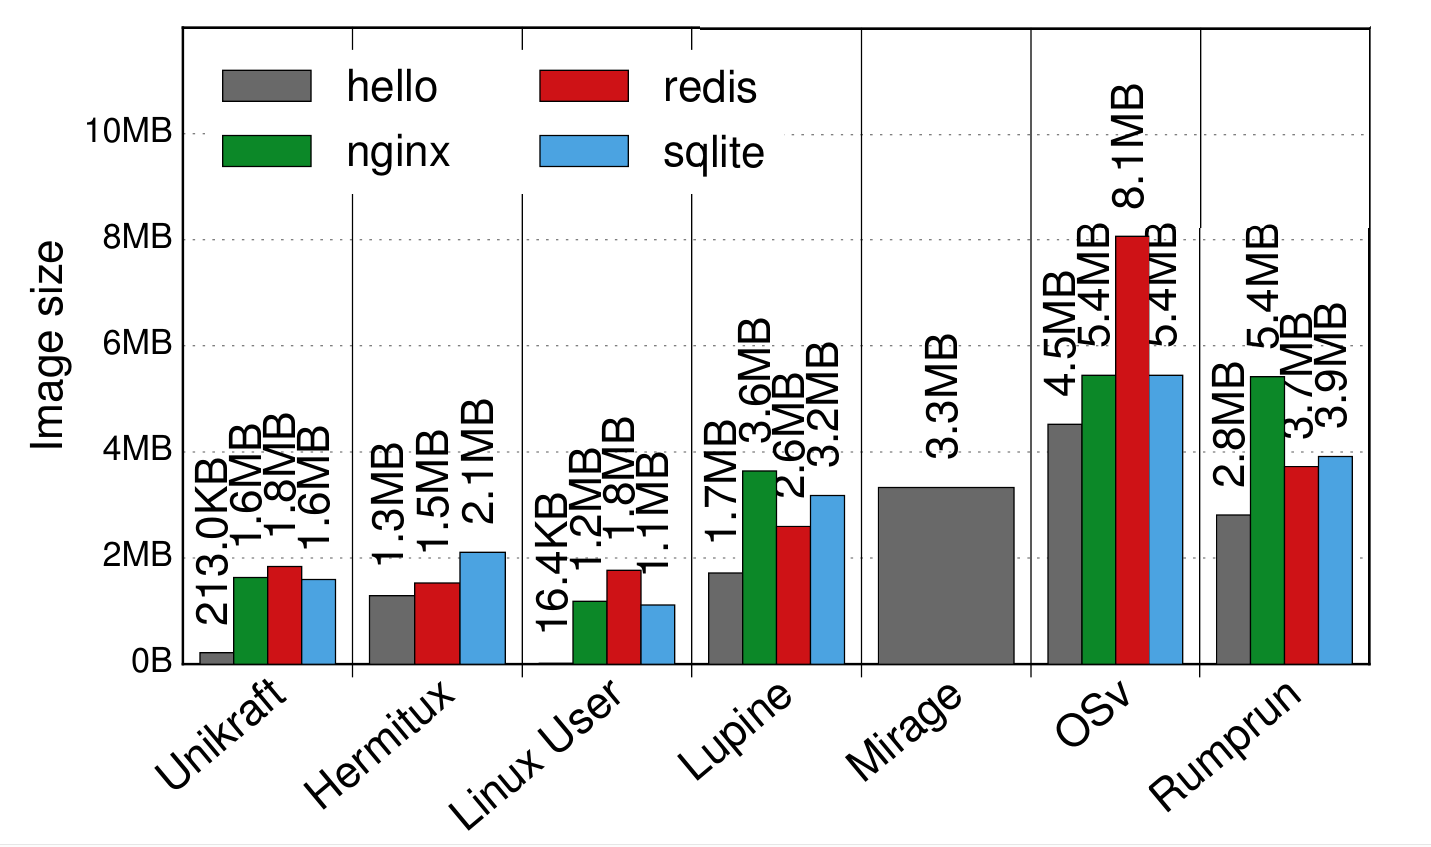
\includegraphics[width=1\linewidth]{pictures/Unikraft-image-size.png}
\caption{}
\label{fig:unikraft-image-size}
\end{minipage}
\begin{minipage}{0.32\linewidth}
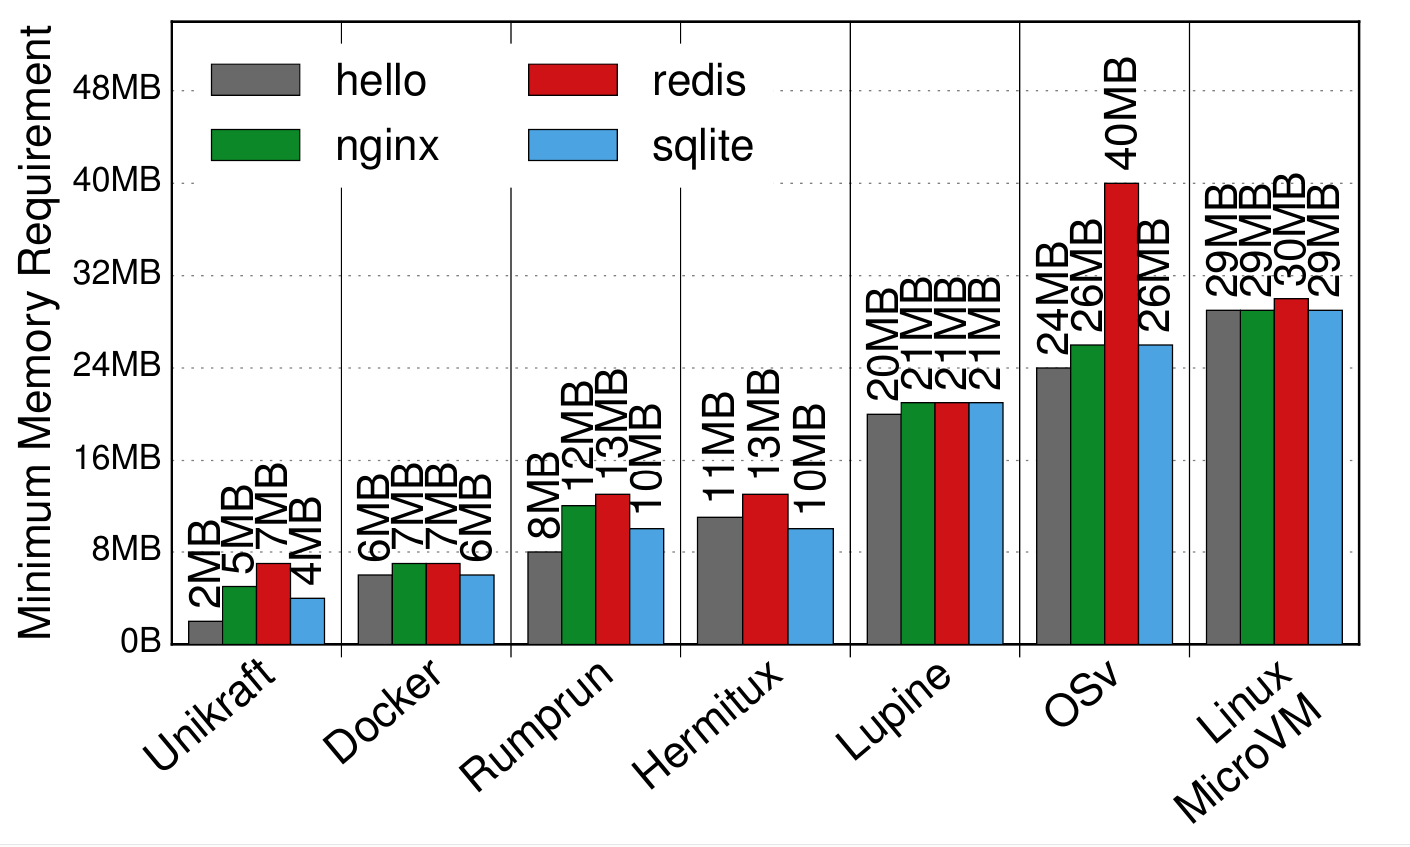
\includegraphics[width=1\linewidth]{pictures/Unikraft-memory.png}
\caption{}
\end{minipage}
\begin{minipage}{0.32\linewidth}
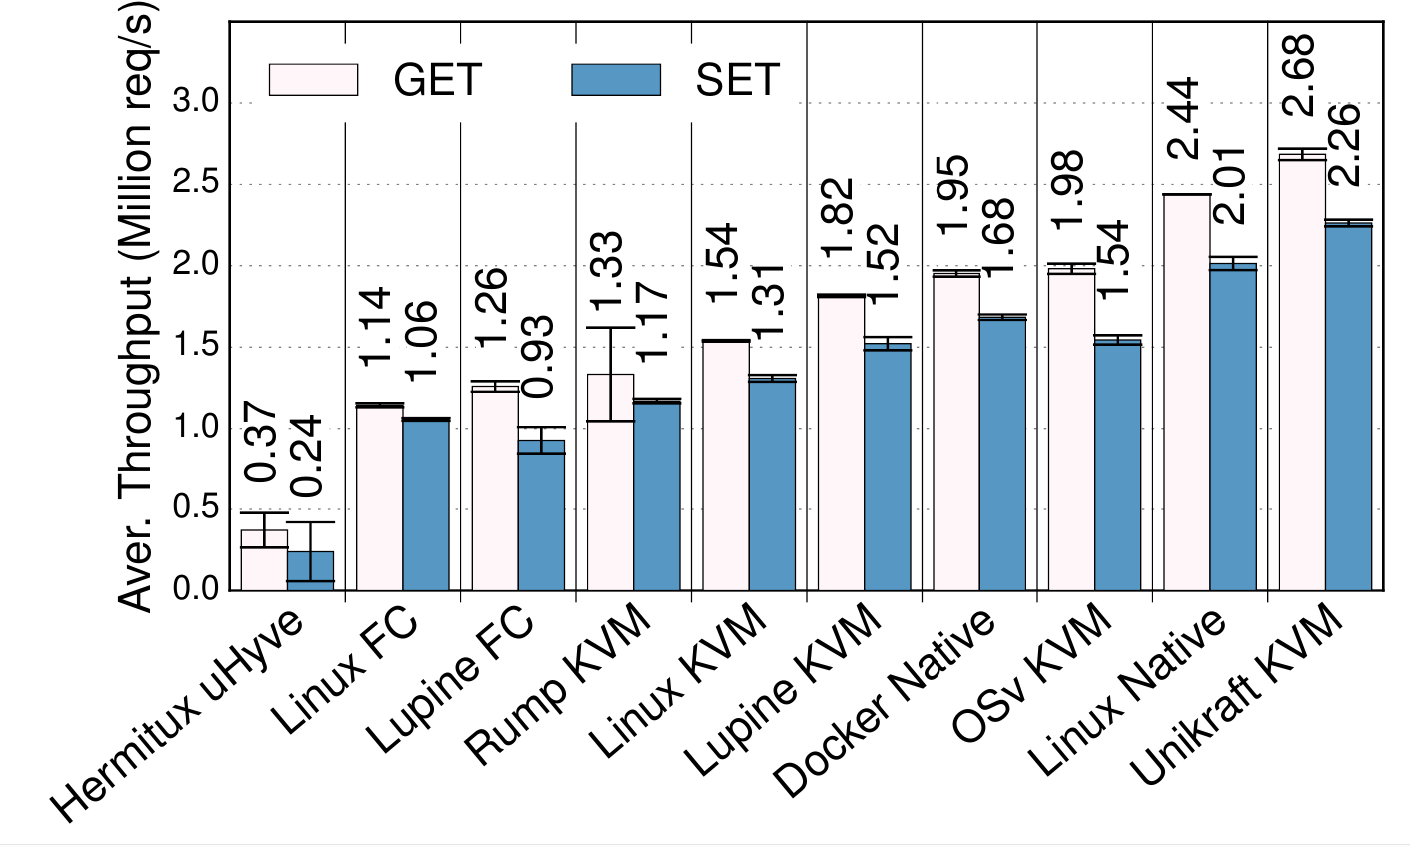
\includegraphics[width=1\linewidth]{pictures/Unikraft-throughput.png}
\caption{}
\end{minipage}
\end{figure}

Unikraft在提升效率的同时兼顾了安全性。根据NCC Group\cite{bib:unikernel-secuirty},
虽然 unikernel 相比容器体积更小、隔离性更好,但是由于不存在内核态-用户态隔离,
且缺乏W\^{}X、stack canary等安全特性,unikernel 其实比传统的容器更不安全。
也就是说,攻击者可以利用 unikernel 上的程序的漏洞,控制 unikernel 所在的虚拟机,
进而未经授权访问资源。
%以 unikernel 的传统应用领域云计算为例,
%如果某个 unikernel 负责处理用户的敏感数据——它通过网络获取用户的数据,
%然后将计算结果通过网络发回,则它一定拥有读用户数据的权限。那么,
%一旦这个 unikernel 存在安全漏洞,攻击者虽然不能控制 unikernel 所在的宿主机,
%但足够窃取用户的数据。
所以,我们不能片面地把安全性与隔离性等同。而且我们不能
片面地认为使用 Rust 这样的安全的程序设计语言就能保证安全,
因为完整的 unikernel 上不只包含安全的系统代码(或者说库代码),还包含可能不安全的用户代码,
而后者可以导致整个系统不安全。因此,要实现安全的 unikernel,不能仅仅依靠安全的程序设计语言,
而需要额外的安全特性。

NCC Group提到了ASLR、分页保护(如W\^{}X政策、内部数据加固、保护页、空页面漏洞等)、
栈保护标志\footnote{它的英文stack canary来自金丝雀曾经被用来检查煤矿的有毒气体的典故\cite{bib:canary}。}、堆加固、标准库加固等安全措施。
%\begin{itemize}
%\item 地址空间布局随机化 (ASLR)。
%\item 分页保护:如W\^{}X政策、内部数据加固、保护页、空页面漏洞。
%\item 栈保护标志(stack canary,典故:金丝雀曾经被用来检查煤矿的有毒气体\cite{bib:canary}):在栈的返回地址后加上一个随机的整型变量(canary),执行\texttt{ret}前检查 canary 是否被修改。
%\item 堆加固:堆的结构通常是双向链表,链表的元数据(如指针)通常与数据块相邻,堆上的溢出可以改变这些数据块,导致内存的分配、释放算法出错,通常的加固方法是为元数据增加校验值。
%\item 熵和随机数生成器:通常的 unikernel 缺乏足够产生密码学安全的伪随机数的硬件熵,这导致 unikernel 上生成的伪随机数的质量差,解决方法有使用 CPU 的专用随机数指令(如 x86 的 \texttt{rdrand})
%\item 标准库加固:如\texttt{printf} 的 \texttt{\%n} 格式符、自定义格式符、\texttt{\_FORTIFY\_SOURCE} 宏。
%\end{itemize}
它测试了 rumprun 和 includeOS 两个 unikernels,并发现它们几乎没有实现任何安全特性。

尽管 Unikraft 使用 C 语言实现,但它支持(或计划支持)
\href{https://github.com/unikraft/unikraft/tree/staging/lib/uksp}{Stack SP}、
\href{https://github.com/unikraft/unikraft/tree/staging/lib/ubsan}{UBSAN}、ARM PAuth、\href{https://github.com/unikraft/unikraft/pull/421}{ARM BTI}、\href{https://github.com/unikraft/unikraft/pull/191}{KASAN}、\href{https://github.com/unikraft/unikraft/pull/239}{PIE}、True Random Number Generator、ARM MTE、
Intel CET、\texttt{FORTIFY\_SOURCE}、ARM SB等安全特性。\cite{bib:unikraft-secuirty}

总的来说,Unikraft是我们发现的最好的unikernel项目,所以我们的项目将
主要参考它。

\subsubsection{比较}

\section{立项依据}\sectionauthor{张子辰}
我们小组计划仿照Unikraft的架构,用Rust语言编写能在RISC-V架构+ QEMU平台上
运行的unikernel——Runikraft。Runikraft的核心代码使用Rust编写,但
允许用户代码使用任何语言编写
%——只要它能够被编译成入口为\texttt{\_start}的目标代码
。Runikraft强调构建系统镜像的简洁,用户只需要
修改现有的项目的编译参数就可以构建基于Runikraft的系统镜像,而不必使用
专用的工具链,更不需要重构代码。Runikraft是POSIX兼容的,所以它将支持
内存管理、进程调度,甚至磁盘管理和进程通信。不过,这些功能都是可选的且可
拓展的,如果用户不需要某项功能,他可以不将相关模块打包进系统镜像中,
如果用户能够提供某些功能的更好实现,他可以用自己的实现替换原有的模块,
甚至POSIX兼容层本身也是可选的,如果用户愿意为了效率重构代码,他也可以
直接用Runikraft的专用API。
Runikraft可以支持多进程,因为我们认为,将若干密切管理的程序打包到一个
镜像会提高效率。
与Unikraft一样,Runikraft在注重效率的同时兼顾安全性。我们计划实现
ASLR、W\^{}X政策、保护页、stack canary四项安全技术。

以往的unikernel项目的不足之处可以概况为(并不每个unikernel都有所有缺点):
\begin{itemize}
\item 无法兼顾效率和兼容性;
\item 系统内的组件耦合度过高,系统不易裁剪或拓展;
\item 需要使用专用的工具构建系统镜像;
\item 将安全性与隔离性等同,忽视了单个unikernel虚拟机的安全;
\item 不支持RISC-V架构;
\item 核心代码使用不安全的程序设计语言编写。
\end{itemize}
而我们的项目将不具有以上缺点。

如果时间允许,我们还会尝试:
\begin{enumerate}
\item 支持更多架构,比如目前流行的AMD64和ARMv8;
\item 支持在裸机上运行,虽然unikernel为云计算诞生,但这并不代表它只适合
    云计算领域,事实上,任何专一用途的设备上的系统都可以是unikernel,
    而且unikernels理论上可以具有比现有的实时系统更高效率;
\item 支持调试,zos小组\textsuperscript{\ref{ssubsec:x-zos}}曾做过相关研究;
\item 移植更多库。
\end{enumerate}

我们考虑过但最终不打算实现与Linux的二进制兼容,即
unipanic\textsuperscript{\ref{ssubsec:x-unipanic}}小组的研究,因为
我们认为不会出现需要移植无法获得源代码的程序的情况:
\begin{itemize}
\item 如果源代码因著作权问题无法获取,那移植二进制文件也会侵犯著作权;
\item 如果源代码因软件无人维护无法获取,那这样的过时软件本身就不应该被继续使用。
\end{itemize}

在系统架构方面,我们将主要参考Unikraft,并少量参考MirageOS和RustyHermit;
在技术方面,我们将参考Chen and Wu的\textit{rCore Tutorial Book}\cite{bib:rcore-os}。
\subsection{Rust语言}\sectionauthor{郭耸霄}

Rust 是由 Mozilla 研究室
主导开发的一门现代系统编程语言,自 2015 年 5 月发布 1.0 之后,一直以每 6 周
一个小版本的开发进度稳定向前推进。语言设计上跟 C++ 一样强调零开销抽象和 RAII。
拥有极小的运行时和高效的 C 绑定,使其运行效率与 C/C++ 一个级别,非常适合对性能
要求较高的系统编程领域。利用强大的类型系统和独特的生命周期管理实现了编译期内存管理,
保证内存安全和线程安全的同时使编译后的程序运行速度极快,Rust 还提供函数式编程语言
的模式匹配和类型推导,让程序写起来更简洁优雅。\cite{bib:2-why-rust}
总地来说,Rust是一门赋予每个人 构建可靠且高效软件能力的语言。\cite{bib:1-rust-lang}
它具有以下三个方面的优越性。

\subsubsection{高性能(Performance)}

Rust 速度惊人且内存利用率极高。由于没有运行时和垃圾回收,它能够胜任对性能要求
特别高的服务,可以在嵌入式设备上运行,还能轻松和其他语言集成。\cite{bib:1-rust-lang}

\begin{itemize}
\item 可执行文件:\\
  Rust是编译语言,这意味着程序直接转换为可执行的机器代码,因此可以将程序作为单个
  二进制文件进行部署;与 Python 和 Ruby 等解释型语言不同,无需随程序一起分发解释器,
  大量库和依赖项,这是一大优势。与解释型语言相比,Rust 程序非常快。\cite{bib:4-rust-go-cmp}

\item 对动态类型语言与静态类型的平衡\\
  动态类型语言在调试、运行时具有不确定性,而静态类型的语言减少了程序理解的开销和动态
  运行的不确定性,但并不是所有静态类型系统都是高效的。Rust的静态类型尽
  最大努力避免程序员的麻烦,同时鼓励长期的可维护性。一些静态类型的语言给程序员带来了沉重的
  负担,要求他们多次重复变量的类型,这阻碍了可读性和重构。其他静态类型的语言允许在全局进行
  数据类型推断。虽然在最初的开发过程中很方便,但是这会降低编译器在类型不再匹配时提供有用的
  错误信息的能力。Rust可以从这两种样式中学习,并要求顶层项具有显式类型,
  同时允许在函数体内部进行类型推断。\cite{bib:3-why-rust-pop}

\item 解决垃圾回收问题\\
  Rust可以选择将数据存储在堆栈上还是堆上,并在编译时确定何时不再需要内存并可以对其进行清理。
  这样可以有效利用内存,并实现更高性能的内存访问。Rust项目非常适合被其他编程语言通过外部功能接口用作库。
  这使现有项目可以用快速的Rust代码替换对性能至关重要的代码,而不会产生其他系统编程语言固有的内存安全风险。
  \cite{bib:3-why-rust-pop}
\end{itemize}

\subsubsection{可靠性(Reliability)}

Rust 丰富的类型系统和所有权模型保证了内存安全和线程安全,让您在编译期就能够消除各种各样的错误。\cite{bib:1-rust-lang}

\begin{itemize}
\item 处理系统级编程\\
  与其他系统级编程语言(例如C或C++)相比,Rust可以提供的最大好处是借阅检查器。
  这是编译器的一部分,负责确保引用不会超出引用的数据寿命,并有助于消除由于内存不安全而导致的
  所有类型的错误。与许多现有的系统编程语言不同,Rust不需要你将所有时间都花在细节上。当安全的Rust无法表达某些
  概念时,可以使用不安全的 Rust。这样可以释放一些
  额外的功能,但作为交换,程序员现在有责任确保代码真正安全。然后,可以将这种不安全的代码包装在
  更高级别的抽象中,以确保抽象的所有使用都是安全的。\cite{bib:3-why-rust-pop}

\item Concurrent programming made easier\\
  Rust makes it easier to write concurrent programs by preventing data races at
  compile time. Rust language can
  check if we are performing any incorrect operations and inform
  us at compile time.\cite{bib:6-why-rust-pop-2}
\end{itemize}

\subsubsection{生产力(Productivity)}

Rust 拥有出色的文档、友好的编译器和清晰的错误提示信息,还集成了一流的工具——包管理器
和构建工具, 智能地自动补全和类型检验的多编辑器支持, 以及自动格式化代码等等。\cite{bib:1-rust-lang}

\begin{itemize}
\item Cargo包管理器\\
  Rust 由于有 Cargo 这样一个非常出色的包管理工具,周边的第三方库发展非常迅速,
  各个领域都有比较成熟的库,比如 HTTP 库有 Hyper,异步 IO 库有 Tokio, mio 等,
  基本上构建后端应用必须的库 Rust 都已经比较齐备。 总体来说,现阶段 Rust 定位的方向
  还是高性能服务器端程序开发,另外类型系统和语法层面上的创新也使得其可以作为开发 DSL
  的利器。\cite{bib:2-why-rust}\\
\end{itemize}
\subsubsection{Rust语言的兼容性}

The Rust language is fast evolving, and because of this certain compatibility
issues can arise, despite efforts to ensure forwards-compatibility wherever possible.

Rust, like many programming languages, has the concept of ``keywords". These
identifiers mean something to the language, and so you cannot use them in places
like variable names, function names, and other places. Raw identifiers let you use
keywords where they would not normally be allowed. This is particularly useful
when Rust introduces new keywords, and a library using an older edition of Rust
has a variable or function with the same name as a keyword introduced in a newer edition.\cite{bib:8-rust-compatibility}

\subsubsection{相比其他语言Rust的优势}

\begin{itemize}
\item Go:Rust语言表达能力更强,性能更高,同时线程安全方面Rust也更强,不容易写出错误的代码,
包管理Rust也更好,Go虽然在1.10版本后提供了包管理,但是目前还比不上Rust的。
\item C++:与C++相比,Rust的性能相差无几,但是在安全性方面会更优,特别是使用第三方库时,
Rust的严格要求会让第三方库的质量明显高很多。语言本身的学习,Rust的前中期学习曲线会更陡峭,
但是对于未来使用场景和生态的学习,C++会更难、更复杂。
\item Java:除了极少部分纯粹的数字计算性能,Rust的性能是全面领先于Java的,同时Rust占用内存小的多,
因此实现同等规模的服务,Rust所需的硬件成本会显著降低。
\item Python:性能自然是Rust完胜,同时Rust对运行环境要求较低,这两点差不多就足够抉择了,
因为python和rust的彼此适用面其实不太冲突。\cite{bib:5-why-rust2}
\end{itemize}

\subsection{RISC-V指令集架构}\sectionauthor{张子辰}
这一部分解释我们为什么要选择RISC-V架构,并且说明RISC-V相比所谓的“成熟”“生态好”
的ARMv8没有任何劣势。

\subsubsection{RISC-V的特点}
RISC-V(“RISC five”)的目标是成为一个通用的指令集架构(ISA):\cite{bib:risc-v-manual}
\begin{itemize}
\item 它要能适应包括从最袖珍的嵌入式控制器,到最快的高性能计算机等各种规模的
处理器。
\item 它应该能兼容各种流行的软件栈和编程语言。
\item 它应该适应所有实现技术,包括现场可编程门阵列(FPGA)
 、专用集成电路(ASIC) 、全定制芯片,甚至未来的设备技术。
\item 它应该对所有微体系结构样式都有效:例如微编码或硬连线控制;顺序或乱序执行
流水线; 单发射或超标量等等。
\item 它应该支持广泛的专业化,成为定制加速器的基础,因为随着摩尔定律的消退,
加速器的重要性日益提高。
\item 它应该是稳定的,基础的指令集架构不应该改变。更重要的是,它不能像以前的
专有指令集架构一样被弃用,例如AMD Am29000、Digital Alpha、Digital VAX、
Hewlett Packard PA-RISC、Intel i860、Intel i960、Motorola 88000、以及Zilog
Z8000。
\end{itemize}

RISC-V的不同寻常不仅在于它是一个最近诞生的指令集架构(它诞生于最近十
年,而大多数其他指令集都诞生于20世纪70到80年代),而且在于它是一个开源的指
令集架构。与几乎所有的旧架构不同,它的未来不受任何单一公司的浮沉或一时兴起
的决定的影响(这一点让许多过去的指令集架构都遭了殃)。它属于一个开放的,非
营利性质的基金会。RISC-V基金会的目标是保持RISC-V的稳定性,仅仅出于技术原
因缓慢而谨慎地发展它,并力图让它之于硬件如同Linux之于操作系统一样受欢迎。

RISC-V的另一个不同寻常之处在于和几乎所
有以往的ISA不同,它是\textit{模块化}的。它的核心是一个名为RV32I的基础ISA,
运行一个完整的软件栈。RV32I是固定的,永远不会改变。这为编译器编写者,操作系统开发人员和汇
编语言程序员提供了稳定的目标。模块化来源于可选的标准扩展,根据应用程序的需要,
硬件可以包含或不包含这些扩展。这种模块化特性使得RISC-V具有了袖珍化、低能耗的特
点,而这对于嵌入式应用可能至关重要。RISC-V编译器得知当前硬件包含哪些扩展后,便
可以生成当前硬件条件下的最佳代码。惯例是把代表扩展的字母附加到指令集名称之后作
为指示。例如,RV32IMFD将乘法(RV32M),单精度浮点(RV32F)和双精度浮点
(RV32D)的扩展添加到了基础指令集(RV32I)中。

\subsubsection{RISC-V的支持}
自诞生以来,RISC-V就得到了Google、华为、IBM、Microsoft、삼성等著名企业\cite{bib:risc-v-manual}和
众多自由软件开发者的支持,所以RISC-V发展迅猛。
尽管历史不长,RISC-V目前已经得到相当完善的软件和硬件方面的支持。
在软件方面,GCC\cite{bib:riscv-gcc}和LLVM\cite{bib:riscv-llvm}都
支持RISC-V架构,这一味着以LLVM为后端的
rustc也支持RISC-V架构。Linux内核自4.15版开设支持RISC-V架构,
到2020年底,Linux 5.10已经支持RISC-V架构的UEFI引导。\cite{bib:riscv-linux}
在Debian发行版中,已经有超过95\%的软件包支持RISC-V架构。\cite{bib:riscv-debian}

在硬件方面,目前已有相当多的RISC-V架构的处理器,比如:\cite{bib:riscv-support}
\begin{itemize}
\item The \href{https://beagleboard.org/beaglev}{BeagleV}, a low-cost single board computer than can run Linux
\item The \href{https://www.sifive.com/boards/hifive1-rev-b}{HiFive1 Rev B} microcontroller
\item The \href{https://www.seeedstudio.com/Perf-V-Based-on-Xilinx-Artix-7-FPGA-RISC-V-opensource-p-4058.html}{Seeed Studio Perf-V} based on a Xilinx Artix-7 RISC-V FPGA
\item The \href{https://www.sparkfun.com/products/15594}{SparkFun RED-V RedBoard}, a microcontroller in an Arduino form factor
\item The \href{https://www.digikey.ca/en/products/detail/groupgets-llc/LOFIVE-R1/10186935}{LoFive} RISC-V SoC evaluation kit
\end{itemize}
\subsubsection{RISC-V的优势}
RISC-V在设计时考虑了成本、简洁性、性能、架构和具体实现的分离、提升空间、
程序大小和易于编程/编译/链接七个因素,并且充分从过去的错误
中吸取了教训:\cite{bib:risc-v-manual}
\begin{longtable}{|p{0.08\linewidth}|*{3}{p{0.27\linewidth}|}}
\hline
&ARM-32 (1986)&x86-32 (1978)&RV32I (2011)\\\hline
\endhead
成本&必须支持整数乘除法&
8 位以及 16 位操作、必须支持整数乘除法&
无 8 位、16 位操作、可选的整数乘 除 法 支 持(RV32M)\\\hline
简洁性&
无零寄存器、条件指令执行、复杂的寻址模式、栈操作指令(push/pop)、算术/逻辑指令中存在移位&
无零寄存器、复杂的过程调用指令(enter/leave)、栈指令(push/pop) 、复杂寻址模式、
循环指令&
  寄存器 x0 专门
  用于存放常数 0、
  立即数只进行符
  号扩展 、一种数
  据寻址模式、没
  有条件执行、没
  有复杂的函数调
  用指令以及栈指
 令、算术指令不
 抛异常、使用单
 独的移位指令来
 处理移位操作\\\hline
性能&
分支指令使用条
 件码、在不同格
 式的指令中,源
 和目的寄存器的
 位置不同、加载
 多个计算得到的
 立即数、 PC 是一
 个通用寄存器&
 分支指令使用
  条件码、每个指
  令中最多只能
  使用两个寄存
  器&
使用同一条指令
实现比较及跳转
(不使用条件
码)、每条指令三
个寄存器 、不能
一次 load 多个数
据、不同指令格
式中,源及目的
寄存器字段位置
固定、立即数是
常数(不是由计
算得出的)、PC
不是通用寄存器\\\hline
架构和具体实现的分离&
将 PC 像 普 通 寄
 存器一样读写,
 这样暴露了流水
 线长度&
 寄存器不是通
  用
 的
  (AX,CX,DX,
  DI,SI 有 特 殊 用
 途)&
不是通用寄存器
 分支指令没有延
 迟槽、Load 指令
 无延迟槽、通用
 寄存器\\\hline
提升空间&
有限的指令码空间&
&
大量可用的指令
码空间位指令位\\\hline
程序大小&
仅 有 32bit 指 令
 (Thumb-2 是一个独立的ISA)&
 仅 32bit 指 令&
 32 位 指 令 +16 位
 RV32C 扩展\\\hline
易于编程/编译/链接&
仅 15 个寄存器、
 内存数据必须对
 齐、不规则的数
 据寻址模式、不
 一致的性能计数
 器&
  仅 8 个通用寄存器、
  内存数据必须
  对齐、不规则的
  数据寻址模式、
  不一致的性能
  计数器&
 31 个寄存器、数
 据可用不对齐、
 PC 相对的数据
 寻址模式 、对称
 的数据寻址模
 式、定义在架构
中的性能计数器\\\hline
\end{longtable}

而且,从学习成本上看,RISC-V相比ARMv8和AMD64也有明显的优势:
RISC-V的“规范”只有4卷,238\cite{bib:riscv-spec1}+155\cite{bib:riscv-spec2}+141\cite{bib:riscv-spec3}+80\cite{bib:riscv-spec4}=614页,
AMD64的“程序员手册”有5卷,3273页\cite{bib:amd64-manual}\footnote{这是AMD提供的手册,
Intel提供的手册更长,有4卷,4830页\cite{bib:amd64-manual-intel}},ARMv8的“参考手册”更是
长达11卷,11530页\cite{bib:armv8-reference}。按两分钟读一页,一天工作八小时,一周工作五天计算,
读完RISC-V的手册需要不到三天,读完AMD64的手册需要将近三周,而读完AMDv8的手册需要两个多月。

\subsection{Unikernel}
Unikernel是专一用途的、单地址空间的轻量操作系统。Unikernels在虚拟机
上运行时,能够提供比传统的容器更短的启动时间、更高的运行效率和更强的
隔离性,因此unikernels通常被用在云计算领域。\cite{bib:unikernel}
然而,为了追求轻量性,
unikernels裁剪了传统的操作系统的众多组件,因此unikernels无法提供许多
常用的库的应用程序接口,所以为了将现有的程序移植到某个unikernel平台,开发者
不得不根据该unikernel的API重构程序。\cite{bib:unikraft}
此外,为了轻量、快速,unikernels
删去的许多基本的并且不会影响性能的安全措施,这导致unikernels相比容器
更容易受到用户程序的安全漏洞的影响。\cite{bib:unikernel-secuirty}

\noindent 目前已经有很多 Unikernel 项目,它们的实现方式大致可以分为两种:
\begin{itemize}
\item 全新的方式(Clean-slate):在构建单一用途的操作系统的假设下,
自由地使用现代工具来进行构建,比如模块化(modularity)、
声明性代码(declarative code)、避开样板文件(avoiding boilerplate)等。
并且从头开始思考操作系统和应用程序层的实现,
使用高级语言进行系统库的编写,从而使得实现更加可掌控,得到的系统库质量更高。
用 OCmal 语言编写的 MirageOS 就是使用 Clean-slate 方式实现的。
\item 传统的方式(Legacy):在不进行修改或只进行一些小的修改的前提下,
运行现有的软件。这通常通过将现有的操作系统代码库重构到库操作系统中来实现。
用 C 语言编写的 Rumprun 是使用 Legacy 方式实现的。
\end{itemize}

\noindent 现有的unikernels普遍存在以下问题:\cite{bib:unikraft}
\begin{itemize}
\item 编译它们并让它们达到高效率需要大量专业的工作,而且这些工作通常
需要对每个目标应用程序重做。
\item 它们通常不是POSIX兼容的,需要移植程序和语言环境。
\end{itemize}

\ref{subsec:famous-unikernel-projects}\ 小节将简要介绍我们小组详细调研的ClickOS、MirageOS、IncludeOS、Rusty-Hermit、Rumprun
和Unikraft等六个目前仍然在维护的unikernel项目。


\section{前瞻性/重要性分析}\sectionauthor{张子辰}
Rust和RISC-V都是新兴事物,并且它们都是在吸取旧事物的教训的基础上诞生的,
而且,实践表明,两者都正在经历蓬勃的发展,并正在分别逐步取代旧事物。
而unikernel本身也是比较新颖的操作系统结构,它在云计算领域正在逐步取代
传统的容器,并且有在嵌入式领域取代传统的嵌入式实时系统的潜能。
因此,用Rust在RISC-V上开发unikernel顺应了历史的趋势。

此外,我们在开发的Runikraft将努力避免现有的unikernels的缺点,集中现有的unikernels
的优点,所以,Runikraft在unikernel领域内部也属于新事物,它将能促进unikernel的发展。
\section{相关工作}
\subsection{安全容器}
\subsection{嵌入式系统}
\subsection{实时系统}
\subsection{用Rust编写的操作系统}

\begin{comment}
\subsection{往年Unikernel项目}\sectionauthor{吴骏东}
本小节介绍往年的操作系统原理与设计(H)课程的与unikernel有关的项目,
以体现我们的项目的独特之处。

\subsubsection{x-unipanic小组}\label{ssubsec:x-unipanic}

\paragraph{1. 项目简介}~\par

该项目旨在已有项目的基础上,小组希望在保持 Unikernel 现有优势(高效、安全、轻量)
的前提下,改善 Unikernel 对二进制程序的支持,做出可以即时打包、分发的 Unikernel。
目前致力于提供二进制兼容性的 Unikernel 项目 \textbf{HermiTux} 仍有较大改进空间,
因此该小组将改善 \textbf{HermiTux} 二进制兼容性作为立项目标。

关键词:UniKernel, 进程调度

参考项目:\href{https://github.com/ssrg-vt/hermitux}{HermiTux}

\paragraph{2. 项目可行性分析}~\par

\begin{itemize}
\item 目前的 Unikernel 实现均要求对应用的重构,在实际应用中无法获取
程序源码、程序依赖未被支持等问题非常常见
\item 将应用打包为 Unikernel 要求大量的专业知识,步骤繁琐
\item HermiTux设计了一个二进制分析工具,能够扫描一个可执行文件,
并检测该程序可以进行的各种系统调用
\item HermiTux基于\href{https://github.com/hermitcore/rusty-hermit}{hermitcore}
这一Unikernel架构做了二进制支持,并重写syscall以保证性能。
\item HermiTux的内核中实现了一个基本的RAM文件系统——MiniFS,从而在这方面消除了对主机的依赖。
\end{itemize}

\paragraph{3. 项目困难点分析}~\par

\begin{itemize}
\item 如果无法获得程序源代码,重新编译和链接将无从进行,
也就不可能打包到 Unikernel。对二进制文件的逆向往往会因为编译过程中
的剥离和混淆难以进行,因此用unikernel层进行拆解和重新链接是不合适的。
\item 让 Unikernel 支持某种语言十分困难,Unikernel 通常只支持一小部分
的内核特性和软件库。如果语言用到了不支持的内容,就需要重写应用,很多情况下
这意味着应用完全不可能被移植。
\item Unikernel 使用复杂的构建工具,将一些传统应用的大型构建基础架构
(大量的 Makefile、autotools/cmake 环境)加入 Unikernel 工具链是十分麻烦。
并且,unikernel还缺乏一些开发工具,如调试器(debugger)和分析工具(profiler)。
\end{itemize}

\paragraph{4. 项目成果分析}~\par

​该小组主要参照了KylinX和Hermitux这两个项目。KylinX项目提供实现fork的思路;
Hermitux主要实现Unikernel的二进制支持,可以在Hermitux的源码上进行改动。主要的成果有:
\begin{enumerate}
\item 支持fork。参照了KylinX实现fork的方式,通过复制hypervisor启动新的
虚拟机作为子进程。但是这样实现的性能较低,增大了系统负担。
\item 优化重写syscall。修改了syscall打包的判断方式,将向后打包扩展成向前打包,
从而100\%重写了syscall函数。保持Unikernel因没有系统调用而具有的优良运行速度。
\end{enumerate}

\subsubsection{x-KATA-Unikernel 小组}

\paragraph{1. 项目简介}~\par

该项目利用 Unikernel 得天独厚的轻量和攻击面小的特性,结合虚拟化技术,
为FaaS(Function As A Service)场景下的云服务提出一种解决方案:
从客户端提交代码,到云平台进行 Serverless 运算。采用 KVM 的虚拟机
接口,在虚拟化环境中以 Unikernel 减少资源开销,达到空间的高效利用和
速度的极限提升。

关键词:UniKernel, 虚拟化, 云计算

参考项目:\href{https://github.com/kata-containers/kata-containers}{Kata}、
\href{https://github.com/google/gvisor/blob/master/README.md}{gVisor}、
\href{https://firecracker-microvm.github.io/}{Firecracker文档}

\paragraph{2. 项目可行性分析}~\par

\begin{itemize}
\item Firecracker 是在 rust 众多 crates 基础上实现的 VMM。
它拥有非常有限的设备模型,提供轻量级的服务并且暴露的攻击面极小,
在 FaaS 场景下有极大的应用空间。但其本质上还是传统的虚拟机架构,不可避免地带来多层嵌套的性能损耗。
\item  Google 提出的 gVisor 解决方案, 在容器的后端将所有的系统
调用截断,凭借 gVisor 中用户程序来实现系统调用的API。 gVisor 极其轻量,
隔离性相对不足。此外,其也面临着过多系统调用时无法忍受的上下文转换问题。
并且,gVisor 采用了带有 GC 的 Go 语言编写,也有比较大的性能开销。
\item Unikernel 的缺点可以被 kata Container易于分发的优点改善,
同时纳入 kubernetes 生态,使得 Unikernel 的应用更加广泛。
\item KVM 是采用硬件虚拟化技术的全虚拟化解决方案。其优势有:依赖
Linux 内核的内存管理、存储和客户机镜像格式多样、支持实时迁移与状态保存、
支持高性能I/O接口、性能极强等。
\end{itemize}

\paragraph{3. 项目困难点分析}~\par

\begin{itemize}
\item Unikernel 的迁移问题。虽然 Unikernel 的概念被提出很久,
市面上也涌现很多 Unikernel 的具体实现,但要找到易于适配 KVM,并且功能齐全的
 core,是一件比较困难的事情。[项目使用了 Nanos解决]
\item 虚拟机对象问题。缺少统一的方式定义虚拟机的各种可管理对象。[项目使用了 libvirt 相关工具解决]
\item 人机交互问题。与客户端的交互需要将虚拟机内部的结果重定向到主机,
此过程中对结果的保护和加密是十分重要的。但这需要较多的知识积累。
\end{itemize}

\paragraph{4. 项目成果分析}~\par

该小组针对当前常用的两种解决方案 Firecracker microVM 和
 gVisor 进行了改造与借鉴,利用 Firecracker 基于 KVM 和
 virIO 的架构获得优异的封装和性能提升,同时希望借鉴 gVisor
 系统调用截断的方式,使其与 Unikernel 进行交互,取代 gVisor
 中 sentry+gofer 的类内核架构,从而达到轻量高效的目的。相关成果如下:

\begin{enumerate}
\item 使用了支持多种语言环境的 Nanos 内核,以 KVM 作为 Unikernel 的载体。
\item 分离 Nanos 的编译编排工具 ops 中的 build 模块,对虚拟机进行硬件加速。
\item 封装 libvirt API ,从而可以更加方便地创建与管理虚拟机。
\item 使用 virt-viewer 工具实现了虚拟机可视化。
\end{enumerate}

改造后的 Unikernel 在算法性能上相较于传统 Linux 提升了约40\%。
后续还可以将 Nanos 进一步与 Firecracker 结合,microVM 与
 Unikernel 的结合可以将性能发挥到极限。

\subsubsection{x-orz小组}

\paragraph{1. 项目简介}~\par

该项目将一般网络程序中的任务看作各种(并发的)基本服务的组合,
抽象出一些常用的服务并让每个 Unikernel 与一个服务相对应,
构成Unikernel实例的集群。通过合理地编排调度 Unikernel 集群,
将各种并发的服务组合起来,处理任务请求,从而充分利用多核/多CPU资源,
提高系统性能,同时又不破坏 Unikernel 原有的轻量、安全的特性。

关键词:Unikernel, 云计算, 高性能计算

参考项目:\href{https://github.com/firecracker-microvm/firecracker}{Firecracker}、
 x-Doudou

\paragraph{2. 项目可行性分析}~\par

\begin{itemize}
\item Unikernel 省去了上下文切换、进程管理、资源竞争等工作带来的开销,
但这样无法充分利用多核尤其是多 CPU 的资源。单个 Unikernel 进程通常仅使用一个核。
支持多核的 Unikernel 往往需要引入OS中有关进程管理、资源分配的复杂模块,
这样便会破坏 Unikernel 的高精简度。
\item 小规模的多进程任务可以将其修改为多线程从而装入同一个 Unikernel 。
但大规模任务只能启动更多的 Unikernel 实例,从而造成相同模块的重复使用。
\item 服务的拆分提高了系统容错性。因为一个 Unikernel 实例相当于一个虚拟服务器,
它的崩溃不会影响整个任务的执行,调度系统只需要再创建/调度另一个提供同样服务的 Unikernel 即可。
\item Firecracker 是一个由AWS开发的轻量级 Hypervisor,旨在加速他们的Serverless服务。
其仅实现了五种必要的I/O设备:virtio-net、virtio-block、virtio-vsock、串口、键盘,
而且它的的启动过程也更为简单,省去了实模式加载等步骤,有着显著的性能提升。
\end{itemize}

\paragraph{3. 项目困难点分析}~\par
\begin{itemize}
\item 相关 OSv 内核的管理工具大部分是为虚拟机或容器开发的,不容易保留原本
OSv+Firecracker 方案的优势(如冷启动时间)。
\end{itemize}

\paragraph{4. 项目成果分析}~\par

该小组参考研究了工业控制系统的结构。其大体的工作流程是在
Interface 部分利用传感器等采集信号,然后通过 Information
Processing 部分进行信息的处理,最后在 Intelligence 部分对
系统进行智能控制。该项目选取了其中的信息处理部分的一小部分,
将应用进行解耦与模块化。将相对独立的功能封装进 Unikernel 运行,
来发挥 Unikernel 快速,安全,轻量的优点,满足相应需求。相关成果如下:
\begin{enumerate}
\item  选用支持多种语言的 OSv 作为 Unikernel 内核,
并在此基础上对 OSv 中相关参数进行了修改,从而提升了 CPU 性能。
\item 使用 Go 语言实现一个轻量的 OSv 管理工具 Uigniter,
功能包括创建、启动、停止 OSv 实例。详细内容见\href{https://github.com/richardlee159/uigniter/tree/e1c063341d658ec897a029b30874bc01bb852a1a}{Uigniter 文档}。
\end{enumerate}

Unikernel 的解决方案具有容器方案所没有的隔离性、安全性、
多进程/线程方案所没有的低延迟、轻量性、高容错率与模块解耦的特性,
在未来 IoT 互联领域有着相当不错的前景。

\subsubsection{X-Doudou 小组}

\paragraph{1. 项目简介}~\par

该项目设计并初步实现了一个面向开发人员和系统管理人员的平台 Cunik ,
用于方便地构建、分发、运行、管理 Unikernel 应用。Cunik 的设计目标
是克服 Unikernel 配置难、部署繁琐的缺点,同时发挥 Unikernel 隔离性好、
性能优良的特点,使运维人员轻松地获益于 Unikernel 这一新兴的技术。

关键词: Unikernel 、虚拟化、容器化

参考项目:libvirt、Rumprun 、OSv

\paragraph{2. 项目可行性分析}~\par

\begin{itemize}
\item Unikernel 在保持了原有的安全性、隔离性、易部署性
的前提下,还做到了在启动速度、运行速度、内存开销等方面全面胜过
 Docker。Unikernel 可以在不同的硬件平台上用不同的方法实现
 不同的应用程序,现在 Unikernel 正运行在世界各地的研究实验室、
 服务器机房以及各种低功耗设备上。
\item Cunik 向用户隐藏繁琐的细节,使用户可以轻松地构建、分发、
获取和配置 Unikernel 应用,降低开发、部署和运维成本,并可以克服
Unikernel 开发难度高、分发部署困难、对系统管理人员要求高、对现有
云计算架构改动大的缺点。借助 Unikernel 的优势,Cunik 可以使用户
轻松获得显著的性能提升和更高的安全性、减小攻击面、降低资源占用。

\item libvirt 提供了便捷且功能强大的虚拟机管理工具。可以基于
 libvirt 构建 Cunik-engine 的 VM Backends 和 VM Hypervisor
  部分从而方便管理虚拟机。
\end{itemize}

\paragraph{3. 项目困难点分析}~\par

\begin{itemize}
\item 需要基于现有的 Unikernel 应用重新开发所需要的平台。
\end{itemize}

\paragraph{4. 项目成果分析}~\par

该小组通过 Python 完成了 Cunik-engine 和 Cunik-cli 的设计,并手动制作了包含 nginx(Rumprun)、redis(Rumprun) 和 redis(OSv) 的本地镜像仓库,
用 Cunik 成功运行了这三种应用。最终在 redis(OSV) 这个应用上取得了比 Linux 上的原生进程更高的性能。

\begin{figure}[!hbt]
\centering
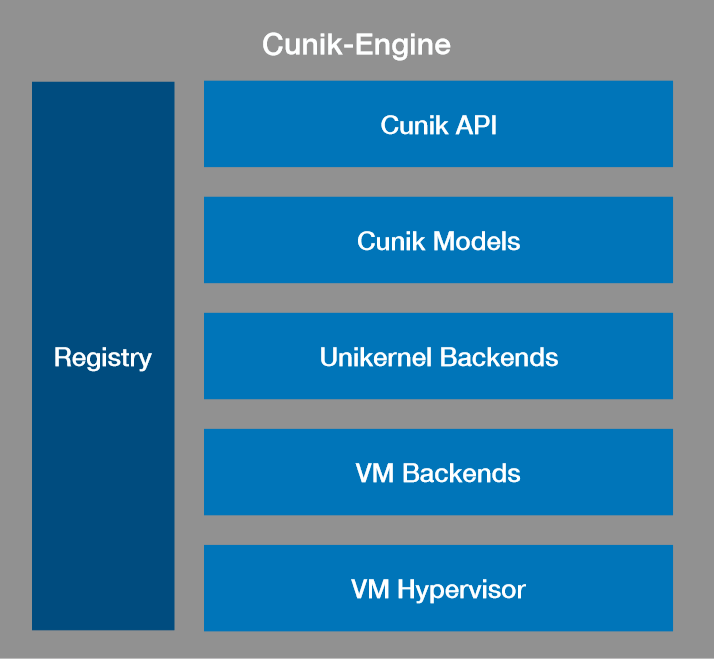
\includegraphics[width=0.5\linewidth]{pictures/resp1.png}
\caption{Cunik-engine 架构}
\end{figure}
其具体细节可参考
\href{https://github.com/OSH-2018/X-Doudou/tree/master/concluding-report}{X-Doudou文档}。
调用 Cunik 后,程序会执行如下的内容:

\begin{enumerate}
\item 用户通过调用 Cunik API 中的 Creat、Run、Stop、
Remove、Inspect 等 API 接口命令来启动 Cunik-engine。
\item Cunik-engine 在接受到命令后,首先会生成一个 Cunik
Config,用于生成 Cunik Object。
\item 通过Cunik Models,engine 会生成 Cunik Object,并加入到
Cunik Registry 中,或对已有 Cunik Object 进行运行状态的修改。
\item 然后,Unikernel Backends 会根据不同的 Cunik Object
选择不同的 Unikernel 实现方式。
\item 接下来,根据所选择的 Unikernel 实现方式,并在 Image Regsitry
中查询 Unikernel 应用的 image ,然后由 VM Backends 生成 VM Config。
\item VM Hypervisor 接收 VM Config 并选择合适的虚拟机来运行这个
Unikernel 应用。
\end{enumerate}

该项目目前只实现了对 kvm/qemu 虚拟机、Rumprun 和 OSv 两种 Unikernel 实现的简单支持。可以改进的内容包括:
\begin{itemize}
\item 整理当前 Cunik-engine 的架构;
\item 实现对更多虚拟机平台以及 Unikernel 实现的支持;
\item 持续支持新的 Unikernel 实现,并加入更多方便
镜像打包与应用部署的特性,使其能够满足生产环境的需要;
\item 更好的交互体验:实现在用户发出 Request 后,
自动为用户选择最合适的一系列 Cunik 应用,达成从前端到后端的一键式搭建服务。
\end{itemize}

\subsubsection{ X-zos 小组}\label{ssubsec:x-zos}

\paragraph{1. 项目简介}~\par

该项目设计了一个利用系统自带的虚拟网卡,通过socket和多线程
并发收发调试信息的日志式调试系统 Umonitor,为运维人员对
Unikernel的调试和维护工作提出了更为轻松有效的解决方案。用户在
使用时只需在每个需要调试的 Unikernel 里调用工具中的 \texttt{send\_log()}
函数,将想要得到的调试信息传入函数,然后在主机的环境里面启动一个host 端,host 端就能通过虚拟网卡接口接收到来自不同 Unikernel 的调试信息并整理保存。

关键词: Unikernel、调试

参考项目: Rumprun

\paragraph{2. 项目可行性分析}~\par
\begin{itemize}
\item 传统的调试手段在 Unikernel 上难以进行。包括:
    \begin{itemize}
    \item 通过与其他进程通信来进行追踪和调试\\
        Unikernel 为了实现精简,而放弃了原有的很多功能,
        其中就包括多进程切换。没有了多进程,就无法利用与其他进程通信来进行debug。
    \item 编程过程中将信息输出在控制台或者文件中\\
        在实际运行 Unikernel 的时候是不会模拟显示器的,
        所以无法将调试信息输出到控制台。又因为 Unikernal 的文件系统
        做了很大的精简,没有VFS,而且不同 Unikernal 的文件系统设计也
        不完全一样,所以,我们如果将日志写入文件,就很难再将虚拟磁盘中的东西读出来。
    \end{itemize}
\item Unikernel 采用了比较原始的单地址空间方式,这可以简化了调试的难度。
单地址空间有助于定位需要的信息在的位置,而并不会影响 Unikernel 的性能。
\end{itemize}
\paragraph{3. 项目困难点分析}~\par
\begin{itemize}
\item 可能实现的方案选择很多,包括文件I/O,串口通信,网络通信等。如何选择最合适的方案需要一定的时间与试错成本。本实验最终选择了通过网络完成unikernel向host发送日志信息的过程。
\end{itemize}

\paragraph{4. 项目成果分析}~\par

该小组设计的 Umonitor 已经可以在 rumpkernel 的平台上通过对
Unikernel 源代码的修改,通过网络通信的方式将 Unikernel 中我们
想要的调试信息输出到制定文件中,初期制定目标已经达到。项目的优势包括:

\begin{enumerate}
\item  \textbf{并发性}:只需启动一个host端就能服务复数的
Unikernel 而无需多开,提高了效率;
\item \textbf{兼容性}:避开了不同的 Unikernel 的差异性,如使用的语言,
内存空间,文件系统等的不同,选择了它们的共性,对 socket 的支持作为实现方法,
几乎所有的 Unikernel 都能无难度地移植这个调试系统;
\item \textbf{高度可控可定制化}:直接在运行 Unikernel 的虚拟机的模拟
vga 输出界面打印调试信息会造成很大的切换和检索的麻烦,而重定向 vga
输出信息至某个文件会输出非常多 Unikernel 自带对调试无用或者不够清晰的信息,
不能得到一个组织良好的日志文件。此外,多个 Unikernel 并发重定向在某些情况下
可能造成输出混杂,不能正确地输出文件。利用 socket 传递自己想要的调试信息并
组织保存,能够生成用户自己最需要的最有用的日志文件,提高调试的效率。
\end{enumerate}

项目可以改进的方向包括:
\begin{enumerate}
\item Unikernel 的调试工具必然需要提供一个通用的接口以实现
对不同种类 Unikernel 的支持。目前的 Umonitor 已经实现了能同时
对多个 Unikernel 的调试,所以下一步的目标可以是实现对多种 Unikernel 的通用接口。使其够方便的支持现阶段较为成熟的 Unikernel 实现的同时
也能够通过用户友好的配置界面对其他 Unikernel 进行支持。
\item Umonitor 在运行之后实际上仍然只能被动地接受被调试的 Unikernel
输出的调试信息,这样虽然能够在一次设置后找到对应的错误信息出现的位置,
但想要在 Unikernel 运行中途添加调试信息输出或者更进一步的设置断点和
逐句执行都还做不到。可以考虑添加交互式调试功能。
\end{enumerate}
\end{comment}

\section*{许可协议}
本文档以知识共享署名 4.0 国际 (CC BY 4.0)许可证发布。

\vspace{2ex}
\noindent\textbf{\large 您可以自由地}:
\begin{description}
\item[共享] 在任何媒介以任何形式复制、发行本作品;
\item[演绎] 修改、转换或以本作品为基础进行创作
在任何用途下,甚至商业目的。
\end{description}

\vspace{2ex}
\noindent\textbf{\large 惟须遵守下列条件}:
\begin{description}
\item[署名] 您必须给出适当的署名,提供指向本许可协议的链接,
同时标明是否(对原始作品)作了修改。您可以用任何合理的方式来署名,
但是不得以任何方式暗示许可人为您或您的使用背书。
\item[没有附加限制] 您不得使用法律术语或者技术措施,从而限制其他人
做许可协议允许的事情。
\end{description}

\vspace{2ex}
\noindent\textbf{\large 声明}:

您不必因为公共领域的作品要素而遵守许可协议,或者您的使用被可适用的例外或限制所允许。

不提供担保。许可协议可能不会给与您意图使用的所必须的所有许可。
例如,其他权利比如形象权、隐私权或人格权可能限制您如何使用作品。

本许可证的全文位于:\\
\centerline{\url{https://creativecommons.org/licenses/by/4.0/legalcode.zh-Hans}}


\begin{thebibliography}{99}
\bibitem{bib:unikernel}
\textit{Unikernels: Rethinking Cloud Infrastructure}[Z/OL].
@unikernel [2022-02-18]. \url{https://web.archive.org/web/20220218194213/http://unikernel.org/}

\bibitem{bib:unikraft} Simon Kuenzer, Vlad-Andrei Bădoiu, Hugo Lefeuvre, Sharan Santhanam,
Alexander Jung, Gaulthier Gain, Cyril Soldani, Costin Lupu, \c{S}tefan Teodorescu, Costi Răducanu,
Cristian Banu, Laurent Mathy, Răzvan Deaconescu, Costin Raiciu and Felipe Huici.
\textit{Unikraft: Fast, Specialized Unikernels the Easy Way}[J/OL]. EuroSys '21, 2021, April: 26–29
[2022-03-27]. \url{https://dl.acm.org/doi/10.1145/3447786.3456248} \texttt{doi:10.1145/3447786.3456248}.

\bibitem{bib:unikernel-secuirty} Spencer Michaels and Jeff Dileo. \textit{Assessing Unikernel Security
}[R/OL]. Version 1.0. NCC Group, 2019: 4-10 [2022-03-27].
\url{https://research.nccgroup.com/wp-content/uploads/2020/07/ncc_group-assessing_unikernel_security.pdf}

\bibitem{bib:1-rust-lang} \textit{Rust Programming Language}[G/OL]. [2022-03-26]. \url{https://web.archive.org/web/20220326232949/https://www.rust-lang.org/}
\bibitem{bib:2-why-rust} @程序师视野. \textit{我们为什么要选择小众语言 Rust 来开发软件?}[Z/OL]. 程序师. [2017-06-26]. \url{https://web.archive.org/web/20170626061304/https://www.techug.com/post/why-we-choose-rust-to-dev.html}
\bibitem{bib:3-why-rust-pop}
Jake Goulding. \textit{What is Rust and why is it so popular?}[Z/OL]. Stack Overflow Blog. 2020 (20200120) [2022-03-24]. \url{https://web.archive.org/web/20220324021421/https://stackoverflow.blog/2020/01/20/what-is-rust-and-why-is-it-so-popular/}
\bibitem{bib:4-rust-go-cmp} CharyGao. \textit{也许是最客观、全面的比较 Rust 与 Go:都想把 Rust 也学一下}[Z/OL]. 博客园. 2020 (20201207) [2022-03-29]. \url{https://web.archive.org/web/20220329090604/https://www.cnblogs.com/Chary/p/14097609.html}
\bibitem{bib:5-why-rust2} 黄光星. \textit{为什么要使用 Rust 语言?Rust 语言的优势在哪里?}[Z/OL].
2020 (20200513) [2022-03-29] \url{https://www.zhihu.com/question/393796866}
\bibitem{bib:6-why-rust-pop-2} Krzysztof Wróbel. \textit{Rust programming language - what is rust used for and why is so popular?}[Z/OL]. codilime, 2022 (20220325) [2022-03-25]. \url{https://codilime.com/blog/why-is-rust-programming-language-so-popular/}
\bibitem{bib:7-rust-by-num} Pavan Belagatti.[\textit{Rust by the Numbers: The Rust Programming Language in 2021}[Z/OL]. The New Stack. 2021 (20210512) [2022-03-25]. \url{https://thenewstack.io/rust-by-the-numbers-the-rust-programming-language-in-2021/}
\bibitem{bib:8-rust-compatibility} \textit{Rust By Example}[M/OL]. Compatibility [2022-03-26]. \url{https://web.archive.org/web/20220326130141/https://doc.rust-lang.org/rust-by-example/compatibility.html}

\bibitem{bib:risc-v-manual} David Patterson and Andrew Waterman. \textit{RISC-V 手册: 一本开源指令集的指南}[S]. 勾凌睿, 黄成, 刘志刚译. 2018: 13-21
\bibitem{bib:riscv-support} Jeff Tranter. \textit{What is RISC-V and Why is it Important?}[Z/OL]. ICS. 2021 (20210512) [2022-03-27]. \url{https://www.ics.com/blog/what-risc-v-and-why-it-important}
\bibitem{bib:riscv-gcc} \textit{Using the GNU Compilers Collections (GCC)}[G/OL]. 2021: RISC-V Options [2022-03-27]. \url{https://gcc.gnu.org/onlinedocs/gcc-11.2.0/gcc/RISC-V-Options.html#RISC-V-Options}
\bibitem{bib:riscv-llvm} \textit{Clang command line argument reference: Clang 15.0.0git documentation}[G/OL]. 2022: RISCV [2022-03-27] \url{https://clang.llvm.org/docs/ClangCommandLineReference.html#riscv}
\bibitem{bib:riscv-linux} Drew Fustini. \textit{Linux on RISC-V
with Open Hardware}[Z/OL]. Embedded Linux Conference, 2020 [2022-03-27]. \url{https://elinux.org/images/3/3d/Linux_riscv_elce2020.pdf}
\bibitem{bib:riscv-debian} \textit{RISC-V}[G/OL]. Debian Wiki, 2022 (2022-03-24) [2022-03-27]. \url{https://wiki.debian.org/RISC-V?action=recall&rev=151}

\bibitem{bib:riscv-spec1} \textit{The RISC-V Instruction Set Manual
Volume I: Unprivileged ISA}[S/OL]. Editors Andrew Waterman and Krste Asanović. Version 2.1. RISC-V Foundation, 2019 (20191213) [2022-03-25]. \url{https://github.com/riscv/riscv-isa-manual/releases/download/Ratified-IMAFDQC/riscv-spec-20191213.pdf}
\bibitem{bib:riscv-spec2} \textit{The RISC-V Instruction Set Manual
Volume II: Privileged Architecture}[S/OL]. Editors Andrew Waterman, Krste Asanović and John Hauser.
Version 1.9.1. RISC-V International, 2021 (20211204) [2022-03-27]. \url{https://github.com/riscv/riscv-isa-manual/releases/download/Priv-v1.12/riscv-privileged-20211203.pdf}
\bibitem{bib:riscv-spec3} \textit{RISC-V Debug Support
}[S/OL]. Editors Ernie Edgar and Tim Newsome. Version 1.0.0-Stable. SiFive, Inc., 2022(20220209)[2022-03-27]. \url{https://github.com/riscv/riscv-debug-spec/raw/b659d7dc7f578e1a2a76f9e62a5eec0f2d80045c/riscv-debug-stable.pdf}
\bibitem{bib:riscv-spec4} \textit{RISC-V Processor Trace}[S/OL]. Gajinder Panesar and
Iain Robertson. Version 1.0. UltraSoC Technologies Ltd., 2020(20200320)[2022-03-27]. \url{https://github.com/riscv/riscv-trace-spec/raw/e372bd36abc1b72ccbff31494a73a862367cbb29/riscv-trace-spec.pdf}

\bibitem{bib:amd64-manual} \textit{AMD64 Architecture Programmer's Manual: Volumes 1-5}[S/OL]. Revision 4.04, Advanced Micro Devices, Inc., 2021 (202111) [2022-03-27]. \url{https://www.amd.com/system/files/TechDocs/40332.pdf}
\bibitem{bib:amd64-manual-intel} \textit{Intel\textsuperscript{®} 64 and IA-32 Architectures Software Developer’s Manual}[S/OL]. Order Number: 325462-076US, Intel Corporation, 2021 (202112) [2022-03-27]. \url{https://cdrdv2.intel.com/v1/dl/getContent/671200}

\bibitem{bib:armv8-reference} \textit{Arm\textsuperscript{®} Architecture Reference Manual
for A-profile architecture}[S/OL]. Version 21.0, Arm Limited, 2022 [2022-03-27]. \url{https://developer.arm.com/documentation/ddi0487/latest}

\bibitem{bib:12-clickos} Joao Martins, Mohamed Ahmed, Costin Raiciu, Vladimir Olteanu,
Michio Honda, Roberto Bifulco and Felipe Huici. \textit{ClickOS and the Art of Network Function Virtualization}[C/OL]. 11th USENIX Symposium on Networked Systems
Design and Implementation. Seattle: USENIX Association. 2014: 459-473[2022-03-22]. \url{http://cnp.neclab.eu/projects/clickos/clickos.pdf}
\bibitem{bib:13-clickos2} Joao Martins, Mohamed Ahmed, Costin Raiciu and Felipe Huici.
\textit{Enabling Fast, Dynamic Network Processing with ClickOS}[J/OL]. HotSDN'13, 2013, August: 67-72[2022-03-22]. \url{http://cnp.neclab.eu/projects/clickos/clickos-workshop.pdf}

\bibitem{bib:11-unikerel2} Anil Madhavapeddy and David J. Scott. \textit{Unikernels: Rise of the Virtual Library Operating System}[J/OL]. ACM Queue, 2014, 11 [2022-03-22].  \url{https://queue.acm.org/detail.cfm?id=2566628}

\bibitem{bib:9-includeos}  Bratterud et al. \textit{IncludeOS: A minimal, resource efficient unikernel for cloud systems}[G/OL]. Adrian Colyer, The morning paper: a random walk through Computer Science research. 2016 (20160222) [2022-03-22]. \url{https://blog.acolyer.org/2016/02/22/includeos}
\bibitem{bib:10-includeos2} Nur Hussein. \textit{IncludeOS: a unikernel for C++ applications}[Z/OL]. 2017 (20170725) [2022-03-22]. \url{https://lwn.net/Articles/728682/}

\bibitem{bib:14-rusty-hermit} \textit{RustyHermit - A Rust-based, lightweight unikernel}[G/OL]. rusty-hermit 0.3.10. [2022-03-25]. \url{https://docs.rs/crate/rusty-hermit/0.3.10}
%\bibitem{bib:15-rust-runtime} Jason 于航. \textit{Rust Runtime 与 ABI}[M/OL]. 知乎专栏, 2021 (20210509) [2022-03-25] \url{https://zhuanlan.zhihu.com/p/370897059}
%\bibitem{bib:16-rust-runtime2} \textit{The Rust runtime}[G/OL]. The Rust Reference. [2022-03-17].
%\url{https://web.archive.org/web/20220317124224/https://doc.rust-lang.org/reference/runtime.html}
\bibitem{bib:17-rusty-hermit2} @stlankes. \textit{The \texttt{RustyHermit} Unikernel}[Z/OL]. Rust OSDev. 2021 (20210122) [2022-03-25]. \url{https://rust-osdev.com/showcase/rusty-hermit/}

\bibitem{bib:18-intra-unikernel} Mincheol Sung and Pierre Olivier. \textit{Intra-Unikernel Isolation with Intel Memory Protection Keys}[C/OL]. 16th ACM SIGPLAN/SIGOPS International Conference on Virtual Execution Environments. Lausanne: Association for Computing Machinery, 2022. \texttt{doi:10.1145/3381052.3381326}.
\bibitem{bib:19-mpk} \textit{Memory Protection Keys}[G/OL]. The Linux Kernel, 5.17.0. [2022-03-18]. \url{https://web.archive.org/web/20220318143208/https://www.kernel.org/doc/html/latest/core-api/protection-keys.html}
%\bibitem{bib:20-linux-kernel} Huo的藏经阁. \textit{linux内核那些事之Memory protection keys(硬件原理)}[Z/OL]. CSDN博客. 2021 (20211119) [2022-03-25]. \url{https://blog.csdn.net/weixin_42730667/article/details/121386896}
\bibitem{bib:21-rump-kernel} Wikipedia Contributors. \textit{Rump kernel}[G/OL]. Wikipedia, 2021 (20210903) [2022-03-29]. \url{https://en.wikipedia.org/w/index.php?title=Rump_kernel&oldid=1042218732}
\bibitem{bib:22-xen} Antti Kantee. \textit{Xen on Rump Kernels and the Rumprun Unikernel}[Z/OL]. XenProject, 2015 (20150806) [2021-08-18].  \url{https://web.archive.org/web/20210818101601/https://xenproject.org/2015/08/06/on-rump-kernels-and-the-rumprun-unikernel/}

\bibitem{bib:23-mirageos} Mircea Cosbuc. \textit{All About Unikernels: Part 2, Two Different Approaches, MirageOS and Rumprun}[Z/OL]. Container Solutions, 2020 (20200125) [2022-01-27]. \url{https://web.archive.org/web/2021*/https://blog.container-solutions.com/all-about-unikernels-part-2-mirageos-and-rumprun}
\bibitem{bib:24-rumrun} Sebastian Wicki. \textit{The Rumprun Unikernel}[Z/OL]. pkgsrcCon, 2016
[2022-03-25]. \url{https://pkgsrc.org/pkgsrcCon/2016/rumprun.pdf}
\bibitem{bib:canary} Wikipedia contributors. \textit{Sentinel species}[G/OL]. Wikipedia, 2022 (20220319) [2022-03-24]. \url{https://en.wikipedia.org/w/index.php?title=Sentinel_species&oldid=1078038868}
\bibitem{bib:unikraft-secuirty} \textit{Unikraft's Inherent Security Benefits}[Z/OL]. Unikraft, 2022 [2022-03-29]. \url{https://web.archive.org/web/20220329100701/https://unikraft.org/docs/features/security/}
\bibitem{bib:rcore-os} Yu Chen and Yifan Wu. \textit{rCore Tutorial Book}[M/OL]. Version 3,
2022(20220102) [2022-03-27]. \url{https://rcore-os.github.io/rCore-Tutorial-Book-v3/chapter0/0intro.html}
\end{thebibliography}
\end{document}